%% Follow comments to support use.

%%%%%%%%%%%%%%%%%%%%%%%%%%%%%%%%%%%%%%%%%%%%%%%%%%%%%%%%%
%% STEP 1: Choose options for MSc / BSc / seminar layout and your bibliographic style
%%%%%%%%%%%%%%%%%%%%%%%%%%%%%%%%%%%%%%%%%%%%%%%%%%%%%%%%%

%%  Language: 
%%      finnish, swedish, or english
%%  Pagination (use twoside by default)  
%%      oneside or twoside,
%%  Study programme / kind of report
%%      csm  = Master's thesis in Computer Science Master's Programme;
%%      tkt = Bachelor's thesis in Computer Science Bachelor's Programme;
%%      seminar = seminar report
%%  For Master's thesis choose your line or track:
%%      (30 cr thesis, 2020 onwards, Master's Programme in Computer Science = csm)
%%      software-track-2020 = Software study track
%%      algorithms-track-2020 = Algorithms study track
%%      networking-track-2020 = Networking study track

\documentclass[english,twoside,censored,csm,algorithms-track-2020,draft]{HYthesisML}


% If wanted, open new chapters only at right page.
% By default, "openany".
%\PassOptionsToClass{openright,twoside,a4paper}{report}
\PassOptionsToClass{openany,twoside,a4paper}{report}

\usepackage{csquotes}
%%%%%%%%%%%%%%%%%%%%%%%%%%%%%%%%%%%%%%%%%%%%%%%%%%%%%%%%%
%% REFERENCES
%% Some notes on bibliography usage and options:
%% natbib -> you can use, e.g., \citep{} or \parencite{} for (Einstein, 1905); with APA \cite -> Einstein, 1905 without ()
%% maxcitenames=2 -> only 2 author names in text citations, if more -> et al. is used
%% maxbibnames=99 as no great need to suppress the biliography list in a thesis
%% for more information see biblatex package documentation, e.g., from https://ctan.org/pkg/biblatex 

%% Reference style: select one 
%% for APA = Harvard style = authoryear -> (Einstein, 1905) use:
\usepackage[style=numeric-comp,backend=biber,natbib=true,maxbibnames=99,giveninits=true,uniquename=init,safeinputenc,sorting=none]{biblatex}
%% for numeric = Vancouver style -> [1] use:
%\usepackage[style=numeric,bibstyle=numeric,backend=biber,natbib=true,maxbibnames=99,giveninits=true,uniquename=init]{biblatex}
%% for alpahbetic -> [Ein05] use:
%\usepackage[style=alphabetic,bibstyle=alphabetic,backend=biber,natbib=true,maxbibnames=99,giveninits=true,uniquename=init]{biblatex}
%

\addbibresource{thesis.bib}
% in case you want the final delimiter between authors & -> (Einstein & Zweistein, 1905) 
% \renewcommand{\finalnamedelim}{ \& }
% List the authors in the Bibilipgraphy as Lastname F, Familyname G,
% \DeclareNameAlias{sortname}{family-given}
% remove the punctuation between author names in Bibliography 
%\renewcommand{\revsdnamepunct}{ }

% Only print URL if no DOI or eprint is given
\DeclareSourcemap{
  \maps[datatype=bibtex]{
    \map{
      \step[fieldsource=doi,final]
      \step[fieldset=url,null]
    }
    \map{
      \step[fieldsource=eprint,final]
      \step[fieldset=url,null]
    }
  }
}


%% Block of definitions for fonts and packages for picture management.
%% In some systems, the figure packages may not be happy together.
%% Choose the ones you need.

%\usepackage[utf8]{inputenc}  % For UTF8 support, in some systems. Use UTF8 when saving your file.


\usepackage{lmodern}         % Font package, again in some systems.
\usepackage{textcomp}        % Package for special symbols
\usepackage[pdftex]{color, graphicx} % For pdf output and jpg/png graphics
\usepackage{epsfig}
\usepackage{subfigure}
\usepackage[pdftex, plainpages=false]{hyperref} % For hyperlinks and pdf metadata
\usepackage{fancyhdr}        % For nicer page headers
\usepackage{tikz}            % For making vector graphics (hard to learn but powerful)
%\usepackage{wrapfig}        % For nice text-wrapping figures (use at own discretion)
\usepackage{amsmath, amssymb} % For better math
\usepackage{algorithm}       % For pseudocode
\usepackage[noend]{algorithmic} % For pseudocode
\usepackage{booktabs}        % For nicer tables
\usepackage{multirow}        % Multirow cells in tables
\usepackage{rotating}        % For sidewaystable

\usepackage[capitalize,noabbrev,nameinlink]{cleveref} % For easier referencing
\Crefname{ALC@unique}{Line}{Lines}
\newcommand{\crefrangeconjunction}{--}


\usepackage{amsthm}          % Theorems
\usepackage{aliascnt}        % Cleveref with shared number theorems
\newtheorem{theorem}{Theorem}[chapter]
\newaliascnt{lemma}{theorem}
\newtheorem{lemma}[lemma]{Lemma}
\aliascntresetthe{lemma}
\newaliascnt{corollary}{theorem}
\newtheorem{corollary}[corollary]{Corollary}
\aliascntresetthe{corollary}
\newaliascnt{proposition}{theorem}
\newtheorem{proposition}[proposition]{Proposition}
\aliascntresetthe{proposition}
\newaliascnt{exercise}{theorem}
\newtheorem{exercise}[exercise]{Exercise}
\aliascntresetthe{exercise}
\newaliascnt{definition}{theorem}
\newtheorem{definition}[definition]{Definition}
\aliascntresetthe{definition}
\newaliascnt{conjecture}{theorem}
\newtheorem{conjecture}[conjecture]{Conjecture}
\aliascntresetthe{conjecture}
\newaliascnt{observation}{theorem}
\newtheorem{observation}[observation]{Observation}
\aliascntresetthe{observation}
\theoremstyle{definition}
\newaliascnt{example}{theorem}
\newtheorem{example}[example]{Example}
\aliascntresetthe{example}
\theoremstyle{remark}
\newaliascnt{note}{theorem}
\newtheorem{note}[note]{Note}
\aliascntresetthe{note}
\newtheorem*{note*}{Note}
\newaliascnt{remark}{theorem}
\newtheorem{remark}[remark]{Remark}
\aliascntresetthe{remark}
\newtheorem*{remark*}{Remark}

% TODO: Remove
\usepackage{lipsum}

\graphicspath{{./plots}}

\singlespacing               %line spacing options; normally use single

\fussy
%\sloppy                      % sloppy and fussy commands can be used to avoid overlong text lines
% if you want to see which lines are too long or have too little stuff, comment out the following lines
% \overfullrule=1mm
% to see more info in the detailed log about under/overfull boxes...
% \showboxbreadth=50 
% \showboxdepth=50



%%%%%%%%%%%%%%%%%%%%%%%%%%%%%%%%%%%%%%%%%%%%%%%%%%%%%%%%%
%% STEP 2:
%%%%%%%%%%%%%%%%%%%%%%%%%%%%%%%%%%%%%%%%%%%%%%%%%%%%%%%%%
%% Set up personal information for the title page and the abstract form.
%% Replace parameters with your information.
\title{MaxSAT-Based Bi-Objective Boolean Optimization}

\author{Christoph Jabs}
\date{\today}

% Set supervisors, use the titles according to the thesis language
% in English Prof. or Dr., or in Finnish toht. or tri or FT, TkT, Ph.D. or in Swedish... 
\supervisors{Prof.~Matti~J\"arvisalo, Dr.~Jeremias~Berg, Dr.~Andreas~Niskanen}

\keywords{Multi-objective optimization, bi-objective optimization, maximum satisfiability, incremental SAT}
\additionalinformation{\translate{\track}}

%% For seminar reports:
%%\additionalinformation{Name of the seminar}

%% Provide classification terms, to appear on the abstract page.
%% Replace the classification terms below with the ones that match your work.
%% ACM Digital library provides a taxonomy and a tool for classification
%% in computer science. Use 1-3 paths, and use right arrows between the
%% about three levels in the path; each path requires a new line.

\classification{\protect{\ \\
\  Mathematics of computing $\rightarrow$ Discrete mathematics $\rightarrow$ Combinatorics $\rightarrow$ Combinatorial optimization \\
\  Theory of computation  $\rightarrow$ Logic $\rightarrow$ Constraint and logic programming
}}

%% If you want to quote someone special. You can comment this line out and there will be nothing on the document.
%\quoting{Bachelor's degrees make pretty good placemats if you get them laminated.}{Jeph Jacques}


%% OPTIONAL STEP: Set up properties and metadata for the pdf file that pdfLaTeX makes.
%% Your name, work title, and keywords are recommended.
\hypersetup{
    unicode=true,           % to show non-Latin characters in Acrobat’s bookmarks
    pdftoolbar=true,        % show Acrobat’s toolbar?
    pdfmenubar=true,        % show Acrobat’s menu?
    pdffitwindow=false,     % window fit to page when opened
    pdfstartview={FitH},    % fits the width of the page to the window
    pdftitle={},            % title
    pdfauthor={Christoph Jabs}, % author
    pdfsubject={},          % subject of the document
    pdfcreator={},          % creator of the document
    pdfproducer={pdfLaTeX}, % producer of the document
    pdfkeywords={algorithms}, % list of keywords for
    pdfnewwindow=true,      % links in new window
    colorlinks=true,        % false: boxed links; true: colored links
    linkcolor=black,        % color of internal links
    citecolor=black,        % color of links to bibliography
    filecolor=magenta,      % color of file links
    urlcolor=cyan           % color of external links
}

%%-----------------------------------------------------------------------------------

\newcommand{\formula}{F}
\newcommand{\Obj}{\textsc{O}}
\newcommand{\inc}{\text{I}}
\newcommand{\dec}{\text{D}}
\newcommand{\var}{\textsc{var}}
\newcommand{\lit}{\textsc{lit}}
\newcommand{\Min}{\texttt{Minimize-\allowbreak{}Inc}}
\newcommand{\Simpr}{\texttt{Solution-\allowbreak{}Improving-\allowbreak{}Search}}
\newcommand{\E}{\texttt{EnumSols}}
\newcommand{\Ex}{\texttt{ExistsSol}}
\newcommand{\T}{\mathtt{T}}
\newcommand{\assumps}{\mathcal{A}}
\newcommand{\satsolver}{\texttt{isSAT}}
\newcommand{\res}{\text{res}}
\newcommand{\algname}{\textsc{BiOptSat}}
\newcommand{\tot}{\textsc{Tot}}
\newcommand{\ov}[2]{\langle #1 < #2 \rangle}
\newcommand{\ove}[2]{\langle #1 \leq #2 \rangle}
\newcommand{\satunsat}{\texttt{SAT-\allowbreak{}UNSAT}}
\newcommand{\unsatsat}{\texttt{UNSAT-\allowbreak{}SAT}}
\newcommand{\msu}{\texttt{MSU3}}
\newcommand{\I}{\mathcal{I}}
\newcommand{\Act}{\texttt{Act}}
\newcommand{\oll}{\texttt{OLL}}
\newcommand{\msh}{\texttt{MSHybrid}}
\newcommand{\hs}{\texttt{hs}}
\newcommand{\nsamp}{n}
\newcommand{\nfeat}{m}
\newcommand{\nclauses}{k}
\newcommand{\selector}{s}
\newcommand{\noise}{\eta}
\newcommand{\equals}{e}
\newcommand{\nelems}{n}
\newcommand{\nsets}{m}
\newcommand{\setcard}{s}
\newcommand{\elemprob}{p}
\newcommand{\sets}{\mathcal{S}}
\newcommand{\element}{e}
\newcommand{\cover}{\mathcal{C}}
\newcommand{\cost}{c}
\newcommand{\cores}{\mathcal{K}}
\newcommand{\core}{\kappa}
\newcommand{\sol}{\tau}
\newcommand{\scep}{SetCovering-EP}
\newcommand{\scsc}{SetCovering-SC}
\newcommand{\clause}{C}
\newcommand{\softs}{\textsc{S}}
\newcommand{\generalobj}{f}
\newcommand{\nobj}{p}
\newcommand{\feasible}{\mathcal{X}}
\newcommand{\decvar}{x}
\newcommand{\soloone}{\{i_2,\allowbreak d_1,\allowbreak d_3,\allowbreak d_4,\allowbreak \lnot i_1,\allowbreak \lnot i_3,\allowbreak \lnot i_4,\allowbreak \lnot d_2\}}
\newcommand{\solotwo}{\{i_1,\allowbreak i_2,\allowbreak d_1,\allowbreak d_2,\allowbreak \lnot i_3,\allowbreak \lnot i_4,\allowbreak \lnot d_3,\allowbreak \lnot d_4\}}
\newcommand{\solothree}{\{i_2,\allowbreak d_1,\allowbreak d_3,\allowbreak d_4,\allowbreak \lnot i_1,\allowbreak \lnot i_3,\allowbreak \lnot i_4,\allowbreak \lnot d_2\}}
\newcommand{\solcone}{\{i_1,\allowbreak i_2,\allowbreak i_3,\allowbreak i_4,\allowbreak d_1,\allowbreak d_2,\allowbreak d_3,\allowbreak d_4\}}
\newcommand{\solctwo}{\{i_1,\allowbreak i_2,\allowbreak d_1,\allowbreak d_2,\allowbreak d_3,\allowbreak d_4,\allowbreak \lnot i_3,\allowbreak \lnot i_4\}}
\newcommand{\solcthree}{\{i_2,\allowbreak d_1,\allowbreak d_2,\allowbreak d_3,\allowbreak d_4,\allowbreak \lnot i_1,\allowbreak \lnot i_3,\allowbreak \lnot i_4\}}
\newcommand{\solcfour}{\{i_1,\allowbreak i_2,\allowbreak i_3,\allowbreak d_1,\allowbreak d_2,\allowbreak \lnot i_4,\allowbreak \lnot d_3,\allowbreak \lnot d_4\}}
\newcommand{\solmcstrap}{\{i_1,\allowbreak i_3,\allowbreak i_4,\allowbreak d_1,\allowbreak d_3,\allowbreak d_4,\allowbreak \lnot i_2,\allowbreak \lnot d_2\}}
\newcommand{\TODO}[1]{\textcolor{red}{#1}}
\newcommand{\thr}{\texttt{thr}}
\newcommand{\NP}{$\mathcal{NP}$}

\begin{document}

% Generate title page.
\maketitle

%%%%%%%%%%%%%%%%%%%%%%%%%%%%%%%%%%%%%%%%%%%%%%%%%%%%%%%%%
%% STEP 3:
%%%%%%%%%%%%%%%%%%%%%%%%%%%%%%%%%%%%%%%%%%%%%%%%%%%%%%%%%
%% Write your abstract in the separate file, to be positioned here.
%% You can make several abstract pages (if you want it in different languages),
%% in which case you should also define the language of the abstract,
%% as below.

\begin{otherlanguage}{english}
\begin{abstract}
\NP-hard combinatorial optimization problems arise naturally in many real-world problems.
Due to this, there is a need for non-trivial algorithmic solutions for solving combinatorial optimization.
Many such solutions---ranging from local search over evolutionary algorithms to declarative programming---have been presented for optimization problems with a single objective.
However, real-world problems are often inherently bi-objective.

We present \algname{}, an exact declarative programming approach for finding so-called Pareto-optimal solutions to bi-objective optimization problems.
We use propositional logic as the declarative programming language and seek to extend the progress and success in maximum satisfiability (MaxSAT) solving to two objectives.
The approach can be viewed as an instantiation of the lexicographic method and makes use of a single SAT solver that is preserved throughout the entire search procedure.
\algname{} allows for solving three tasks for bi-objective optimization:
finding a single Pareto-optimal solution, finding one representative solution for each Pareto point, and enumerating all Pareto-optimal solutions.

We provide an open-source implementation and empirical evaluation of five different variants of \algname{}, building on different algorithms known from MaxSAT solving.
We empirically evaluate \algname{}, comparing its runtime performance to three competing algorithmic approaches ($P$-minimal, ParetoMCS and Seesaw), showing practical benefits of our approach in the contexts of learning interpretable decision rules and bi-objective set covering.
Furthermore, for the best-performing variant of \algname{}, we study the effects of proposed refinements to determine their effectiveness.
\end{abstract}
\end{otherlanguage}


% Place ToC
%\newpage
\mytableofcontents

\mainmatter

%%%%%%%%%%%%%%%%%%%%%%%%%%%%%%%%%%%%%%%%%%%%%%%%%%%%%%%%%
%% STEP 4: Write the thesis.
%%%%%%%%%%%%%%%%%%%%%%%%%%%%%%%%%%%%%%%%%%%%%%%%%%%%%%%%%
%% Your actual text starts here. You shouldn't mess with the code above the line except
%% to change the parameters. Removing the abstract and ToC commands will mess up stuff.
%%
%% Command \include{file} includes the file of name file.tex.
%% A new page will be created at every \include command, 
%% which makes it appropriate to use it for large entities such as book chapters. Cannot be nested.
%% It is useful for a big project, as changing one of the include targets 
%% won't force the regeneration of the outputs of all the rest.
%% Alternatively, \input is a more lower level macro 
%% which simply inputs the content of the given file like it was copy&pasted there manually.

\chapter{Introduction\label{chap:intro}}

% Being upfront: What is this thesis about?
In this thesis, we propose an algorithmic approach for solving \NP-hard optimization problems with two conflicting objectives exactly.
The algorithm proposed is based on declarative programming in the paradigm of propositional satisfiability, and is generally applicable to problems that can be easily represented in propositional logic.

% What are optimization problems and where do they occur
% Start by telling a story (running example throughout intro)
When one is looking for a new flat to buy, most people will be comparing prices with the aim to find the cheapest flat possible that fulfils their requirements.
This is an example of what are called optimization problems.
Optimization problems can be summarized as the task of finding a ``best'' solution out of a collection of possible solutions available.
Commonly, the notion of ``best'' that is used in optimization is that a solution of minimum associated ``cost'' is considered optimal.
Speaking in the example from above, the task is to find the flat that fulfils the requirements for the cheapest price.
If the collection of possible solutions is discrete (as in the flat example), we speak of \emph{combinatorial} optimization.

% Applications of optimization in literature
Combinatorial optimization problems naturally arise in many areas, ranging from industrial applications over research to everyday tasks.
Examples in literature include scheduling~\autocites{DBLP:conf/cp/Stojadinovic14,DBLP:conf/cpaior/BofillGSV15,DBLP:journals/ior/Solomon87,DBLP:journals/candie/AkyolB07}, supply chain optimization~\autocite{DBLP:journals/cce/Papageorgiou09}, air traffic management~\autocites{DBLP:journals/ior/BertsimasLO11,RichardsHow2002Aircrafttrajectoryplanning}, clustering~\autocite{DBLP:journals/ai/DaoDV17,DBLP:conf/sdm/DavidsonRS10}, learning optimal classifiers~\autocites{DBLP:conf/cp/MaliotovM18,DBLP:conf/ijcai/NarodytskaIPM18,DBLP:conf/ijcai/Hu0HH20,DBLP:conf/cp/YuISB20,DBLP:conf/aaai/DemirovicS21,DBLP:conf/cp/ShatiCM21,DBLP:conf/cade/IgnatievPNM18} and many more.

% Hardness of optimization problems
In the same way that there are different complexity classes~\autocite{AroraBarak2009-complexity} for decision problems, these complexity classes can be extended to optimization problems as well.
Probably the two most important complexity classes are $\mathcal{P}$ and \NP.
$\mathcal{P}$ contains all problems for which an algorithm that solves the problem in polynomial time is known.
On the other hand, for problems in \NP, currently no such algorithm is known.
This means that the worst case runtime for \NP-complete (i.e., exactly as hard as the hardest problems in \NP) and \NP-hard (i.e., at least as hard as problems in \NP) problems is exponential.
Consider the \NP-complete set covering decision problem~\autocite{DBLP:conf/coco/Karp72} where for a collection $\sets$ of sets, the task is to determine whether a cover $\cover$ with cardinality smaller than a threshold $k$ exists so that the cover intersects all sets, i.e., $S \cap \cover \neq \emptyset$ for all $S\in\sets$.
The corresponding optimization problem, where the task is to find the \emph{smallest} such cover is \NP-hard.
Several well known \NP-complete decision problems have corresponding \NP-hard optimization problems~\autocite{KorteVygen2018-15}.

% Approaches to solving optimization
Since there is such a variety of applications for combinatorial optimization, a plethora of algorithmic approaches to solving optimization problems have been proposed.
These approaches range from local search~\autocite{DBLP:books/daglib/0017492}, over evolutionary~\autocites{DBLP:books/daglib/0087893,DBLP:journals/jgo/StornP97} to declarative programming-based algorithms~\autocite{handbook2-maxsat,ChenEtAl2010-intro,DBLP:reference/fai/2}.
In addition to these generally applicable approaches, there are problem specific algorithms, e.g., based on dynamic programming~\autocite{DBLP:conf/aaai/DemirovicS21}\TODO{more examples}.
One other attribute on which the optimization approaches differ is whether they are exact or approximative, meaning if they are guaranteed to find \emph{the best} or \emph{a good} solution to any instance (given enough resources).
Even though some others are also briefly surveyed in a later chapter, this work focuses on declarative (and therefore general) and exact approaches.

% Solving pipeline for declarative approaches
The declarative programming approach to optimization follows the solving pipeline illustrated in \cref{fig:solving-pipeline}.
First, the problem of interest is \emph{encoded} into a declarative programming language of choice.
Examples of declarative languages are maximum satisfiability~\autocite{handbook2-maxsat}, constraint programming~\autocite{DBLP:reference/fai/2} and mixed integer linear programming~\autocites{ChenEtAl2010-intro,KorteVygen2018-5}.
An encoding is hereby a mapping of each instance of the original problem to an instance in the declarative language, where each optimal solution to the encoded instance corresponds to an optimal solution to the original instance.
A fitting declarative language for a given problem can be chosen so that the problem can be naturally encoded in the language.
Secondly, a general optimization solver for the declarative language is used to solve the encoded problem and obtain on optimal solution for it.
A solver for a declarative programming language is an algorithm that finds an optimal solution to an instance in a declarative programming language.
The last step is to map this solution back to the original problem space.

\begin{figure}
  \centering
  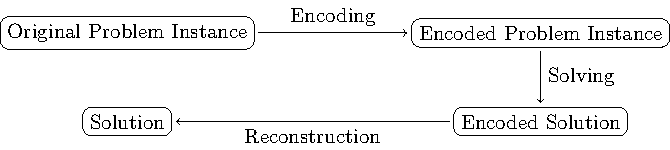
\includegraphics{solving-pipeline.pdf}
  \caption{The solving pipeline of the declarative approach to optimization.}\label{fig:solving-pipeline}
\end{figure}

% Advantages of declarative approaches
The advantage of the declarative approach is that the solving algorithm itself is general and can be used for different original problems, as long as a small enough encoding exists.
The task of applying the declarative method based on a specific language to a new problem consists therefore in finding an encoding and not in coming up with a new algorithm.
Furthermore, improvement that is made in developing solvers for a declarative language immediately maps to better solving performance for \emph{all} problems that can be encoded into this declarative language.

% Runtimes in declarative approaches
In the scope of this work, we focus on using declarative approaches for solving \NP-hard optimization problems.
For this application, \NP-hard declarative languages are used, meaning the generic solving step is the only computationally hard step in the solving pipeline.
Both the encoding and the reconstruction of the solution are typically done in polynomial time.
Since the declarative language is \NP-hard (assuming $\mathcal{P}\neq\mathcal{NP}$), the worst-case runtime of the solving algorithm cannot be better than exponential.
However, in practice one can observe significantly better performance from many solving algorithms for ``interesting'' instances, i.e., instances that appear for real-world problems.
Examples for solving algorithms for \NP-hard declarative languages that achieve good performance on real-world instances are conflict driven clause learning solvers for propositional satisfiability~\autocite{handbook2-cdcl} and state-of-the-art branch-and-cut algorithms for mixed integer linear programming~\autocite{ChenEtAl2010-branch-and-cut}.

% Reveal conflicting second objective
Coming back to the flat search example from the beginning, we can notice a problem emerging:
what does ``fulfilling'' the requirements mean?
Some requirements, like the number of rooms, might be easy to specify, but consider the distance of ones daily commute.
Rather than setting a fixed threshold as ``maximum $d$ kilometres distance'', what we might actually want to do is minimize this distance at the same time as the cost of the flat.
Now there are multiple objectives to take into account regarding what constitutes a ``best'' solution.
Multiple objectives give rise to \emph{multi-objective} optimization.

% Conflicting objectives and why there might be no single optimal solution
A crucial difference between single-objective and multi-objective optimization is that there is no single notion of optimality for the multi-objective setting.
Whereas for a single objective function, there is a clear minimum (or maximum) and objective values can be unambiguously compared, this becomes less defined for the multi-objective case:
consider a flat with a cost of 300\,000 \texteuro{} and 1-kilometre daily commute and compare it to another flat that costs 240\,000 \texteuro{} and has a 3-kilometre daily commute.
It is not immediately clear which one of these options is better, and the choice would depend on ones personal preference over the two objectives.
This becomes especially difficult if there is no clear preference over the objectives.
Typically, a situation like that occurs when two of the objectives considered are in conflict, as the price of a flat and the corresponding daily commute might be if the commute is towards the city centre and flats in the city centre are more expensive.

% Pareto optimality
% Point out different nomenclature
In the context of our work, the notion of optimality for multi-objective optimization is that of Pareto optimality (also called efficiency in other contexts)~\autocite{Ehrgott2005-2}.
Intuitively, Pareto optimality considers a solution optimal if there are no other solutions with better objective values for one objective and not worse for all the others. 
This definition would consider the two last flats from earlier both equally optimal.
Under Pareto optimality, the task of solving a multi-objective optimization problem can mean multiple things:
finding a single Pareto-optimal solution, finding a representative solution for each Pareto point (also called non-dominated point in literature~\autocite{Ehrgott2005-2}), or finding all Pareto-optimal solutions.
Most approaches to solving multi-objective optimization under Pareto optimality seem to focus on the second approach where a single solution per Pareto point (i.e., tuple of Pareto-optimal objective values) is computed.
This gives a human decision maker the ability to look at the results and choose the Pareto-optimal solution that gives the best trade-off between the objectives after the fact instead of having to choose such a trade-off in advance.
The last task goes one step further and enumerates the full Pareto front (i.e., all Pareto-optimal solutions), even if multiple of the solutions might lead to the same objective values.
All three of these tasks can be solved by the algorithmic approach presented in this thesis.

% Bi-objective vs multi-objective
% Why bi-objective is interesting/enough
The handle on multiple objectives and what the objective values of an optimal solution actually mean can quickly become hard to grasp.
As humans, we can only visualize three dimensions, meaning a Pareto front over four objectives is already an entirely abstract object while even a three-dimensional one is hard to visualize.
% Imagine, for example, adding the objectives living space and renovations that need to be done into the flat search example.
% With those four objectives, a lot more flats are going to be Pareto-optimal and the set of Pareto-optimal solutions becomes less helpful for making a decision.
Two objectives, however, form a good trade-off between gaining meaningful information from the second objective over just using a single one, being able to intuitively visualize the Pareto front and not resulting in too many Pareto-optimal solutions.
Additionally, objectives that are considered ``less important'' but should still somehow be included in the optimization can still be added as a threshold condition.
% e.g., requiring that the living space is more than 60 $\text{m}^2$ rather than treating it as a separate objective.

% Applications of bi-objective optimization in literature
Bi-objective combinatorial optimization problems arise naturally in many fields of application.
When learning interpretable classifiers, the objectives ``interpretability'' and ``classification error'' are in conflict.
As a proxy for interpretability, typically a notion of ``size'' of the model is used, leading to a natural bi-objective optimization problem with the objectives ``classification error'' and ``model size''~\autocites{DBLP:conf/ijcai/Ignatiev0NS21,DBLP:conf/cp/MaliotovM18,DBLP:conf/ijcai/NarodytskaIPM18,DBLP:conf/ijcai/Hu0HH20,DBLP:conf/cp/YuISB20,DBLP:conf/aaai/Ignatiev0S021,DBLP:conf/cade/IgnatievPNM18}.
A bi-objective optimization problem also arises when wanting to create a portfolio of different solvers that together solve a set of benchmarks as fast as possible while also containing as few solvers as possible~\autocite{DBLP:conf/cp/JanotaMSM21}.
There are also bi-objective optimization problems in network routing with the objectives load balancing and latency~\autocite{SilverioEtAl2022biobjectiveoptimization}.
In supply chain optimization, in addition to the economic objective, environmental aspects can be taken into consideration as a second objective~\autocites{DBLP:journals/cce/Pinto-VarelaBN11,DBLP:journals/candie/TautenhainBN19}.

% MaxSAT (and SAT)
In this work, we use maximum satisfiability (MaxSAT) as the declarative programming language for solving optimization problems with the declarative approach.
MaxSAT is the \NP-hard optimization variant of the \NP-complete propositional satisfiability (SAT) problem.
It seeks to find an assignment to a given propositional formula, maximizing the number of satisfied clauses.
Solvers for MaxSAT have made significant progress over the recent years and are by now very efficient for solving many practical optimization problems.
This progress is mainly due to development on the underlying SAT solvers used in MaxSAT solving~\autocites{DBLP:journals/ai/FroleyksHIJS21,handbook2-cdcl}, but also due to improved algorithms for how to apply those SAT solvers in MaxSAT solving.

% SAT-based bi-/multi-objective optimization not very active in last years
% Motivation for researching that direction
Approaches for SAT- and MaxSAT-based bi- or multi-objective optimization have been proposed in the past~\autocites{DBLP:conf/cp/SohBTB17,DBLP:conf/ijcai/Terra-NevesLM18a,DBLP:conf/aaai/Terra-NevesLM18,DBLP:conf/ijcai/Terra-NevesLM18,DBLP:conf/cp/JanotaMSM21}, but it is not a very active field of research.
In this thesis, we seek to extend the progress and success in MaxSAT solving to multiple objectives.

% Contributions
% Algorithm: single SAT solver; builds on MaxSAT; single vs all
The main contributions of this work is the \algname{} algorithm, a MaxSAT-based bi-objective optimization approach.
\algname{} builds on advances in MaxSAT solving, allowing for variants based on different solution-improving~\autocites{handbook2-maxsat,DBLP:journals/jsat/BerreP10,DBLP:journals/jsat/EenS06} and core-guided~\autocites{DBLP:journals/corr/abs-0712-1097,DBLP:conf/sat/AnsoteguiBL09,DBLP:conf/cp/MorgadoDM14,DBLP:journals/jsat/IgnatievMM19} algorithms.
We propose five different variants of \algname{}, the first four building on the SAT-UNSAT~\autocite{DBLP:journals/jsat/BerreP10}, UNSAT-SAT~\autocite{DBLP:conf/sat/FuM06}, MSU3~\autocite{DBLP:journals/corr/abs-0712-1097} and OLL~\autocite{DBLP:conf/cp/MorgadoDM14} MaxSAT algorithms.
The fifth variant is a hybrid between SAT-UNSAT search and MSU3, aiming to combine the advantages of the two approaches.
In addition to five variants of \algname{}, we also propose multiple refinements for improving the performance of \algname{}:
lazily building the cardinality constraints for both objectives, blocking dominated solutions, domain-specific blocking, bound hardening and other refinements known from core-guided MaxSAT solving.
\algname{} allows for solving all three tasks for bi-objective optimization:
finding a single Pareto-optimal solution, one representative solution for each Pareto point or enumerating all Pareto-optimal solutions.

% Evaluation: study efficiency of different MaxSAT algorithms
After proposing \algname{}, this thesis empirically evaluates the performance of it on two benchmark domains:
learning interpretable decision rules from binary data~\autocite{DBLP:conf/cp/MaliotovM18} and bi-objective set covering.
In the experiments, we compare all five variants of \algname{} to two SAT-based competitors:
enumeration of $P$-minimal solutions~\autocite{DBLP:conf/cp/SohBTB17} and Seesaw~\autocite{DBLP:conf/cp/JanotaMSM21}.
As a result of this evaluation, we determine which variant of \algname{} is the best-performing overall.
Furthermore, for the best-performing variant, we study the effects of the proposed refinements to determine their effectiveness.

% Signposting for chapters
This thesis is structured as follows:
On overview of propositional satisfiability and maximum satisfiability, highlighting the important preliminaries needed to understand the proposed algorithm, is given in \cref{chap:satisfiability}.
In \cref{chap:biobjective-optimization}, an overview of bi-objective optimization is given, defining the problem and surveying some existing approaches, based on SAT, other declarative paradigms, and probabilistic and meta-heuristic approaches.
After that, in \cref{chap:approach}, \algname{} including five variants and some refinements is proposed.
Finally, in \cref{chap:experiments} we outline the experiments and results, and conclude the thesis in \cref{chap:conclusion}.
\chapter{Propositional Satisfiability\label{chap:satisfiability}}

% Signposting
In this chapter, an overview of propositional satisfiability (SAT) is given.
The first section, defines the SAT decision problem.
In the second section, an overview of incremental SAT solving, a technique that our algorithm makes heavy use of, is given.
Next, we briefly discuss maximum satisfiability, the optimization variant of propositional satisfiability.
The chapter concludes with a section on encoding cardinality constraints in propositional logic.

\section{The Propositional Satisfiability Problem\label{sec:sat}}

% Propositional logic and SAT
For a Boolean variable $v$ there are two literals, the positive $v$ and the negative $\lnot v$. 
A clause $C$ is a set of (disjunction over) literals and a CNF formula $\formula$ is a set of (conjunction over) clauses.
The set of variables and literals appearing in $\formula$ are $\var(\formula)$ and $\lit(\formula)$, respectively.  
A truth assignment $\sol$ maps boolean variables to 1 (true) or 0 (false).
The semantics of truth assignments are extended to a clause $C$ and a formula $\formula$ in the standard way: $\sol(C) = \max\{ \sol(l) \mid l \in C\}$ and $\sol(\formula) = \min\{\sol(C) \mid C \in \formula\}$.
When convenient, we view assignments $\sol$ over a set $\var(\formula)$ of variables as sets of literals $\sol = \{ v \mid v \in \var(\formula),  \sol(v) = 1\} \cup \{ \lnot v \mid v \in \var(\formula), \sol(v) = 0\}$.
An assignment $\sol$ for which $\sol(\formula) = 1$ is a solution to $\formula$.
The propositional satisfiability (SAT) problem asks whether a given formula $\formula$ has a solution.
A formula $\formula$ is satisfiable if it has solutions, otherwise it is unsatisfiable.

% Example: SAT
\begin{example}
  Take the propositional formula $\formula_1 = a \land \lnot b$ over variables $\var(\formula_1) = \{a,b\}$.
  It is satisfiable since the assignment $\sol=\{a,\lnot b\}$ has $\sol(\formula_1)=1$.
  The formula $\formula_2 = a \land \lnot a$ on the other hand is not satisfiable.
\end{example}

% SAT solvers
A SAT solver is an algorithm that determines the satisfiability of a given formula $\formula$.
If the formula is satisfiable, it returns ``satisfiable'' (SAT) and a solution $\sol$ with $\sol(\formula)=1$;
if it is unsatisfiable, it returns ``unsatisfiable'' (UNSAT).

% SAT as a declarative modelling language
\TODO{Extend and explain solving pipeline properly. Maybe move to Intro.}
The SAT problem was proved to be $\mathcal{NP}$-complete in~\textcite{DBLP:conf/stoc/Cook71}.
This result is very central to the modern day use of SAT as a declarative programming approach to solving other $\mathcal{NP}$-complete problems by encoding them as a propositional formula first, solving them with a SAT solver and then decoding the solution to the original problem context.
The advantage of using SAT as a declarative programming language for solving other problems comes from the fact that---even though SAT is $\mathcal{NP}$-complete, and it is unclear if a polynomial time algorithm for solving it exists---conflict-driven clause learning solvers~\autocite{handbook2-cdcl} for SAT are efficient in practice and can solve problems with millions of variables and clauses~\autocite{}.

% Example: SAT modelling
\begin{example}\label{ex:sat-modelling}
  We give an example of a real-world problem, modelling and solving it with the help of SAT.
  Assume you have the following problem:
  you want to plan a meal for a guest coming over and don't know whether to include an appetizer, a main course and a dessert.
  However, you know the following constraints:
  (i)~there must be a main course in every meal, (ii)~having three courses is too much effort, (iii)~your guest would like to have dessert, and (iv)~you have a new appetizer recipe that you would like to try making.
  To model this problem as SAT, you can introduce three variables $v_\text{a}$, $v_\text{m}$, $v_\text{d}$ modelling whether appetizer, main course and dessert are included in the meal.
  With these, the four conditions form the following four clauses:
  $\clause_\text{(i)} = v_\text{m}$, $\clause_\text{(ii)} = \lnot v_\text{a} \lor \lnot v_\text{m} \lor \lnot v_\text{d}$, $\clause_\text{(iii)} = v_\text{d}$, and $\clause_\text{(iv)} = v_\text{a}$.
  Next, you can solve the formula $\clause_\text{(i)} \land \clause_\text{(ii)} \land \clause_\text{(iii)} \land \clause_\text{(iv)}$ with the help of a SAT solver, which will return UNSAT.
  This tells you that there is no choice of the three courses that satisfies all conditions.
  As the host, you could now either put in more work for the meal (removing constraint~(i)) or decide to make the appetizer recipe some time else (removing constraint~(iv)).
  Assume you decide to remove constraint (iv), then the solution to $\clause_\text{(i)} \land \clause_\text{(ii)} \land \clause_\text{(iii)}$ found by the SAT solver is $\sol = \{ \lnot v_\text{a}, v_\text{m}, v_\text{d} \}$.
  Interpreting this solution, you know that making a main course and a dessert, but leaving out the appetizer, satisfies all constraints.
\end{example}

\section{Incremental SAT Solving under Assumptions\label{sec:inc-sat}}

% Incremental SAT solving
It is common that algorithms that solve problems with the help of SAT solvers produce a series of SAT problems that only differ slightly.
To be able to solve these sub-problems more efficiently, most modern SAT solvers provide an incremental interface that allows for retaining information learned in previous solver calls~\autocite{DBLP:journals/entcs/EenS03,handbook2-cdcl}\TODO{ check if new CDCL chapter can be referenced}.
In order for the learned information \TODO{define learned info} from previous solver queries to still hold for subsequent calls, it is only possible to \emph{add} clauses to the solvers internal formula, not remove them.
In addition, incremental SAT solvers support solving under assumptions.
The assumptions $\assump$ are a set of literals that are treated as unit clauses, i.e., a solver call with internal formula $\formula$ and assumptions $\assump$ either returns SAT and a solution $\sol \supset \assump$, or UNSAT and a subset $\core \subset \{\lnot l \mid l\in\assump\}$ such that $\formula \land \bigwedge_{l \in \core} (\lnot l)$ is unsatisfiable.
The subset $\core$ is called an unsatisfiable \emph{core} and, intuitively, is an explanation for the unsatisfiability of the query.

\TODO{Define \texttt{isSAT}.}

\section{Maximum Satisfiability\label{sec:max-sat}}

% MaxSAT
Maximum satisfiability (MaxSAT) is the optimization variant of the SAT decision problem.
In it, the goal is to find a solution that satisfies as many of the given clauses as possible.
Most commonly and in this work, MaxSAT refers to the extension of \emph{weighted partial} MaxSAT, in which a set of \emph{hard} clauses $\formula$ and another set of \emph{soft} clauses $\softs$ are given.
Each clause $\clause \in \softs$ is assigned a weight $w_\clause$ and a solution $\sol$ that satisfies $\formula$ while achieving minimal weight of falsified soft clauses $\sum_{\clause\in\softs \mid \tau(\clause)=0} w_\clause$ is optimal for the problem.

% MaxSAT as a modelling language
In the same way that SAT can be used as a declarative language to solve other decision problems, MaxSAT can be used to solve optimization problems.

% Example: MaxSAT modelling
\begin{example}\label{ex:maxsat-modelling}
  \TODO{Adapt \cref{ex:sat-modelling}, removing constraint (ii), changing it too the objective}
\end{example}

\section{Encoding Cardinality Constraints as Totalizers\label{sec:card-const}}

% Cardinality constraints
A common type of constraint to appear when encoding problems into SAT is that of a cardinality constraint.
Informally speaking, cardinality constraints enforce a bound on how many literals in a set can be assigned to true.
Formally, for a set $L$ of literals and a bound $b \in \mathbb{N}$, $\texttt{As-CNF}\left(\sum_{l \in L} l \circ b\right)$ denotes a CNF formula that encodes the linear inequality $\sum_{l \in L} l \circ b$, where $\circ \in \{< ,> ,\geq, \leq, =\}$.
Numerous methods of forming such CNF formulas are known~\autocite{DBLP:conf/cp/BailleuxB03}\TODO{better reference}.

% Totalizer encoding
In this work we make use of the totalizer encoding.
Given a set $L$ of $n$ input literals and a bound $k=1, \ldots, n$, the (incremental) totalizer~\autocite{DBLP:conf/cp/BailleuxB03,DBLP:conf/cp/MartinsJML14} encoding produces a CNF formula $\tot(L, k)$ that defines a set $\{\ov{L}{1}, \ldots, \ov{L}{k}\} \subset \var(\tot(L))$ of \emph{output literals} that---informally speaking---count the number of literals in $L$ assigned to true by solutions to $\tot(L)$:
if $\tau$ is an assignment that satisfies $\tot(L)$, then $\tau(\ov{L}{b}) = 1$ if $\sum_{l \in L} \tau(l) < b$.
Even though the full totalizer encoding also supports lower bounding the number of literals (in which case we would have $\tau(\ov{L}{b})=1$ \emph{if and only if} $\sum_{l \in L} \tau(l) < b$), since in this work we only use upper bounds, the size of the encoded totalizer can be reduced by leaving the corresponding clauses out.
\TODO{Rewrite previous sentence(s). Possibly first define full totalizers and then discuss reduced variant.}
The incremental totalizer supports both increasing the bound $k$ and adding new input literals without having to rebuild the whole formula:
we have that $\tot(L, k) \subset \tot(L, k')$ and $\tot(L, k) \subset  \tot(L \cup L', k)$ hold for any bound $k' > k$ and set $L'$ of literals for which $L \cap L' =  \emptyset$. 
\TODO{Discuss why this is desirable.}
We use $\ove{L}{k}$ as a shorthand for the literal $\ov{L}{k+1}$.
Note that the assignments of the auxiliary variables of the totalizer encoding are functionally defined by the assignment of the input and output variables.
As such we will leave them out from the solutions we describe in favour of brevity and clarity of examples. 
\chapter{Pareto Optimality and Bi-Objective Optimization\label{chap:biobjective-optimization}}

% Signposting
This chapter describes bi-objective optimization, starting with a definition of the problem and the more general case of multi-objective optimization.
We also define the notation for bi-objective optimization in the context of SAT that is used in this work.
For reference of what other work has been done as well, we give an overview of other notions of optimality for multiple objectives and different approaches to solving bi-objective optimization problems.

\section{Pareto-Optimal Multi-Objective Optimization\label{sec:multiopt}}

% Multiobjective optimization
Multi-objective optimization deals with optimizing $\nobj$ given objective functions $\generalobj_i: \feasible \rightarrow \mathbb{R}^+$ where $i=1,\dots,\nobj$, with the solution $\decvar$, while $\decvar$ is from a feasible set $\feasible$~\autocite{Ehrgott2005-1}.
W.l.o.g., we assume that all objective functions are to be \emph{minimized}.
Formally, a multi-objective optimization problem (MOOP) is of the form:
\begin{equation}\label{eq:moop}
  \min (\generalobj_1(x),\dots,\generalobj_\nobj(x)),\ \text{subject to}\ x\in \feasible.
\end{equation}
The space that the feasible set $\feasible$ is a subset of is called \emph{decision space}.
Every point in the decision space is mapped to a point in \emph{objective space} by the objective functions.

% Pareto optimality
For multi-objective optimization problems, since the objectives might be in conflict with each other (i.e., optimality cannot be reached for all of them at the same time) no single optimal solution exists.
One natural way to define optimality for multiple objectives is Pareto optimality, based on dominated solutions.
\begin{definition}[Dominated Solutions~\autocite{Ehrgott2005-2}]
  Given a MOOP as defined in \cref{eq:moop} and two solutions $x,x' \in \feasible$, $x$ dominates $x'$ (w.r.t.\ $\generalobj_1,\dots,\generalobj_\nobj$) if (i)~$\generalobj_i(x) \leq \generalobj_i(x')$ for all $i=1,\dots,\nobj$, and (ii)~$\generalobj_i(x) < \generalobj_i(x')$ for some $i\in\{1,\dots,\nobj\}$.
  We represent $x$ dominating $x'$ by $x \prec x'$.
\end{definition}
\begin{definition}[Pareto Optimality~\autocite{Ehrgott2005-2}]
  Given a MOOP as defined in \cref{eq:moop}, a solution $x \in \feasible$ is Pareto-optimal (w.r.t.\ $\generalobj_1,\dots,\generalobj_\nobj$) if and only if there is no $x' \in \feasible$ such that $x' \prec x$, i.e., $x$ is not dominated by any other solution.
\end{definition}
When the objectives are clear from context, we will simply say that a solution $x$ is Pareto-optimal.
Note that there can be multiple Pareto-optimal solutions to a MOOP.
The set of all Pareto-optimal solutions is called the Pareto front (w.r.t.\ $\generalobj_1,\dots,\generalobj_\nobj$);
the tuple $(\generalobj_1(x),\dots,\generalobj_\nobj(x))$ for a Pareto-optimal $x$---i.e., the image of $x$ in objective space---is a Pareto point.
Multiple Pareto-optimal solutions can correspond to the same Pareto point.

Multi-objective optimization under Pareto optimality gives rise to three different tasks:
finding (i)~a single Pareto-optimal solution, (ii)~a representative solution for every Pareto point, and (iii)~all Pareto-optimal solutions.
The algorithmic approach proposed in this thesis can be used for solving all three of these tasks, however, we focus on the latter two.

\section{Bi-Objective Optimization in a SAT Context\label{sec:biopt}}

% Bi-objective optimization in a SAT context
In this work, we focus on \emph{bi}-objective optimization, where the number of objective functions is $\nobj=2$.
Furthermore, we work with linear objective functions with integer coefficients, as they can be easily encoded in SAT.
We formalize linear bi-objective optimization in a context of propositional satisfiability in the following way:
An objective $\Obj$ is a multiset of literals, which allows for representing objective functions with non-unit coefficients.
The value $\Obj(\sol)$ of a truth assignment $\sol$ under $\Obj$ is $\Obj(\sol) = \sum_{l \in \Obj} \sol(l)$, i.e., the number of the literals in $\Obj$ that $\sol$ assigns to 1. 
Weighted objectives with integer coefficients are represented by adding a literal multiple times.
Formalizing the objectives this way and encoding the feasible set $\feasible$ as a propositional formula $\formula$ is similar to MaxSAT, where $\formula$ corresponds to the hard clauses while the two objectives correspond to two sets of (unit) soft clauses.

% Example: A bi-objective problem
\begin{figure}
  \begin{minipage}{0.377\textwidth}
    \small
    \begin{align*}
      \formula = &\bigg\{ \texttt{As-CNF}\left(\sum_ {l \in \Obj_\inc \cup \Obj_\dec} l \geq 4 \right), \\
        &(i_1 \lor i_2), (i_2 \lor i_3), (i_2 \lor i_4) \\
        &(d_1 \lor d_2), (d_2 \lor d_3), (d_2 \lor d_4) \bigg\}, \\
      \Obj_\inc =&\{ i_1, i_2, i_3, i_4 \}, \\
      \Obj_\dec =&\{ d_1, d_2, d_3, d_4 \} 
    \end{align*}
  \end{minipage}
  \;
  \begin{minipage}{0.605\textwidth}
    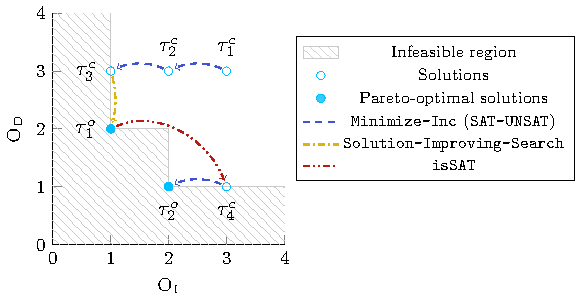
\includegraphics{search-trace.pdf}
  \end{minipage}
  \caption{Left: An example formula $\formula$ and two objectives $\Obj_\inc$ and $\Obj_\dec$.
    Right: the feasible region of $\formula$ in the objective space defined by $\Obj_\inc$ and $\Obj_\dec$.
    The solutions $\tau^o_1$ and $\tau^o_2$ (solid points) are Pareto-optimal, while $\tau^c_i$ for $i=1,\ldots,4$ are not.\label{fig:search-trace}}
\end{figure}
\begin{example}\label{ex:main}
  An example formula $\formula$ and two objectives $\Obj_\inc$ and $\Obj_\dec$ are shown on the left side of \cref{fig:search-trace}. 
  The solution space is illustrated on the right.
  The three solid dots correspond to the three Pareto points of $\formula$ w.r.t.\ $\Obj_\inc$ and $\Obj_\dec$. 
  Examples of Pareto-optimal solutions corresponding to these points are $\sol^o_1 = \soloone$, $\sol^o_2 = \solotwo$ and $\sol^o_3 = \solothree$.
  The solution $\sol^c_3 = \solcthree$ is dominated by $\sol^o_1$ ($\sol^o_1 \prec \sol^c_3$) because $\Obj_\inc(\sol^o_1) \leq \Obj_\inc(\sol^c_3)$ and $\Obj_\dec(\sol^o_1) < \Obj_\dec(\sol^c_3)$. \\
  (The arrows in \cref{fig:search-trace} represent subroutines of \algname{} and will be discussed in \cref{chap:approach}.)
\end{example}

% Proposition: Ordered Pareto front
An important property of Pareto-optimal solutions to bi-objective problems is summarized by the next proposition.
\begin{proposition}[Adapted from~\autocite{DBLP:conf/aaai/HartertS14}] \label{prop:biobjective}
  Sorting the Pareto-optimal solutions of a bi-objective optimization problem under the objectives $\generalobj_1$ and $\generalobj_2$ w.r.t.\ increasing values of $\generalobj_1$ is equivalent to sorting them w.r.t.\ decreasing values of $\generalobj_2$ and vice-versa.
\end{proposition}

% Example: Ordered Pareto front
\begin{example}
  Consider the formula $\formula$, the objectives $\Obj_\inc$ and $\Obj_\dec$ and the three Pareto-optimal solutions $\sol^o_1$, $\sol^o_2$ and $\sol^o_3$ from \cref{fig:search-trace} and \cref{ex:main}.
  By \cref{prop:biobjective}, lowering the value of one objective of a Pareto-optimal solution has to increase the value of the other;
  we have $\Obj_\inc(\sol^o_1) = 1 < \Obj_\inc(\sol^o_2) = 2 < \Obj_\inc(\sol^o_3) = 3$ and $\Obj_\dec(\sol^o_1) = 3 > \Obj_\dec(\sol^o_2) = 2 > \Obj_\dec(\sol^o_3) = 1$.
\end{example}

\section{On Other Notions of Optimality}

% Signposting
As mentioned in \cref{sec:multiopt}, Pareto optimality is only one notion of optimality for multiple objectives.
There are two other important notions of optimality for bi-objective optimization that narrow down the set of solutions that are considered optimal:
lexicographic optimization and lexicographic max-ordering optimization~\autocite{Ehrgott2005-5}.
These notions of optimality can be seen as a way of specifying in advance which Pareto-optimal solutions are of interest.
The solutions considered optimal are a subset of all Pareto-optimal solutions and every algorithm finding all Pareto-optimal solutions will therefore also find all solutions optimal under these other notions.
For this reason, solving multi-objective optimization under these other notions of optimality can be considered easier than solving it under Pareto optimality.
Both lexicographic optimization and lexicographic max-ordering optimization are general for any number of objectives, however, here we describe them in the context of bi-objective optimization.

% Lexicographic optimization
In lexicographic optimization~\autocite{Ehrgott2005-5}, a preference over the objectives is enforced, considering only one of the ``end points'' of the Pareto front---i.e., a Pareto-optimal solution with the smallest value for the objective chosen as primary---optimal.
Formally, given a feasible set $\feasible$ and two objectives $\generalobj_1$ and $\generalobj_2$, a solution $x$ dominates another solution $x'$ in the lexicographic sense if (a)~$\generalobj_1(x) < \generalobj_1(x')$, or (b)~$\generalobj_1(x) = \generalobj_1(x')$ and $\generalobj_2(x) < \generalobj_2(x')$.
Intuitively, we can also say lexicographic optimization asks to compute a solution that minimizes $\generalobj_1$ using $\generalobj_2$ as a tie-breaker.
The comparison criterion can also be seen as lexicographically comparing the string of objective values of two solutions, hence the name of the notion of optimality.

% Example: lexicographic optimization from a perspective of Pareto optimality
\begin{example}
  Consider again the formula $\formula$ and the objectives $\Obj_\inc$ and $\Obj_\dec$ from \cref{fig:search-trace}.
  Assume the objective $\Obj_\inc$ is chosen as the objective with higher priority.
  In this case, all solutions corresponding to the Pareto point $(3,1)$ (e.g., $\sol^o_1 = \soloone$) are lexicographically optimal.
\end{example}

% Lexicographic optimization with the weighted sum method
Lexicographic optimization can be cast into an optimization problem with a single objective with the help of the weighted sum method~\autocite{Ehrgott2005-3}.
This is a common approach to solving lexicographic optimization, since solving algorithms for optimization problems with one objective are widely available for different paradigms.

% Leximax optimization
Lexicographic max-ordering (leximax) optimization~\autocite{Ehrgott2005-5} is closely related to lexicographic optimization.
The only difference is that for leximax optimization, the objective values are sorted in descending order before comparing them lexicographically.
This leads to the Pareto points with the smallest maximum objective value being considered optimal.
Let $\generalobj_\text{max}(x) = \max\{\generalobj_1(x), \generalobj_2(x)\}$ and $\generalobj_\text{min}(x) = \min\{\generalobj_1(x), \generalobj_2(x)\}$.
Formally, a solution $x$ dominates another solution $x'$ in the leximax sense if (a)~$\generalobj_\text{max}(x) < \generalobj_\text{max}(x')$, or (b)~$\generalobj_\text{max}(x) = \generalobj_\text{max}(x')$ and $\generalobj_\text{min}(x) < \generalobj_\text{min}(x')$.
Informally speaking, this notion of optimality seeks to keep all objective values low by minimizing the maximum value first.
All leximax-optimal solutions are contained in the set of Pareto-optimal solutions, however, they might correspond to different Pareto points.

% Example: lexicographic max-ordering optimization from a perspective of Pareto optimality
\begin{example}
  Consider again the formula $\formula$ and the objectives $\Obj_\inc$ and $\Obj_\dec$ from \cref{fig:search-trace}.
  The solution $\sol^o_2 = \solotwo$ is leximax-optimal, since it has the smallest maximum objective value.
\end{example}

\section{Earlier Approaches to Bi-Objective Optimization\label{sec:approaches}}

% Signposting
In this section, we give an overview of different approaches to solving bi-objective optimization problems.
The focus hereby lies on \cref{sec:sat-based}, describing SAT-based approaches.
In the section thereafter, we survey exact approaches based on other declarative optimization paradigms, mainly constraint and mixed integer programming.
\Cref{sec:approximative} gives a brief overview of methods to approximate the Pareto front.
In addition to approaches solving bi-objective optimization under Pareto optimality, we also discuss some approaches that make use of different optimality definitions.

\subsection{SAT-Based Approaches\label{sec:sat-based}}

% Signposting
We highlight three SAT-based approaches to bi-objective optimization under Pareto optimality:
enumeration of $P$-minimal solutions, enumeration of Pareto-minimal correction sets, and Seesaw.
Furthermore, we touch on SAT-based optimization under lexicographic optimality.

\subsubsection{$P$-minimal Solution Enumeration\label{sec:p-minimal}}

% P-minimal solution enumeration
The approach perhaps closest to ours is solving multi-objective constraint optimization problems by enumerating so-called $P$-minimal solutions~\autocites{DBLP:conf/cp/SohBTB17,DBLP:conf/ftp/KoshimuraNFH09}.
This approach corresponds to enumerating the solutions of $\formula^\text{W} = \formula \land \tot(\Obj_{\inc}) \land \tot(\Obj_{\dec})$ that are subset-minimal w.r.t.\ the set of outputs of the totalizers.
More precisely, if $P$ is the set of output literals of $\tot(\Obj_{\inc}) \land \tot(\Obj_{\dec})$, then the goal is to enumerate solutions $\sol^m$ such that no other solution $\sol$ has $\{ l \mid l \in P, \sol(l) = 0\} \subsetneq \{ l \mid l \in P, \sol^m(l) = 0\}$.
The procedure for enumerating such solutions~\autocite{DBLP:conf/ftp/KoshimuraNFH09} works by (i)~using a solver to obtain any solution $\sol$ of $\formula^\text{W}$, (ii)~iteratively minimizing the subset of variables of $P$ set to true by the solution, and, once a minimal solution $\sol_m$ has been found, (iii)~adding the clause $(\ov{\Obj_{\inc}}{k_1} \lor \ov{\Obj_{\dec}}{k_2})$ containing the output variables corresponding to the lowest index set to true by $\sol_m$.
We refer to the algorithm for enumerating $P$-minimal solutions as ``$P$-minimal'' for short.

% Example: P-minimal
\begin{example}\label{ex:pmin}
  Consider the formula $\formula$ and two objectives $\Obj_\inc$ and $\Obj_\dec$ from \cref{fig:search-trace}.
  $P$-minimal starts by building two totalizers $\tot(\Obj_\inc)$ and $\tot(\Obj_\dec)$ and invoking the SAT solver on $\formula^\text{W} = \formula \land \tot(\Obj_\inc) \land \tot(\Obj_\dec)$.
  The result is satisfiable, assume the first solution obtained is $\sol^c_1 = \solcone$. 
  In order to minimize $\sol^c_1$, the clause $(\ov{\Obj_\inc}{4} \lor \ov{\Obj_\dec}{4})$ is added to the SAT solver, and the solver is invoked again under the assumptions $\{ \ove{\Obj_\inc}{4}, \ove{\Obj_\dec}{4} \}$.
  The added clause blocks $\sol^c_1$ and all solutions dominated by $\sol^c_1$ from the search space.
  Assume the next solution obtained is $\sol^c_5 = \solmcstrap$. 
  Again, a clause $(\ov{\Obj_\inc}{3} \lor \ov{\Obj_\dec}{3})$ is added, and the SAT solver is queried with the assumptions $\{ \ove{\Obj_\inc}{3}, \ove{\Obj_\dec}{3} \}$.
  The result is \sat{}, assume the solution obtained is $\sol^o_2 = \soloone$. 
  $P$-minimal then adds the clause $(\ov{\Obj_\inc}{2} \lor \ov{\Obj_\dec}{2})$ and invokes the solver again under the assumptions $\{ \ove{\Obj_\inc}{2}, \ove{\Obj_\dec}{2} \}$.
  The result is \unsat{} which proves that $\sol^o_2$ is Pareto-optimal. 
  To find a next Pareto-optimal solution, the solver is queried without any assumptions for a new solution to start the minimization process from.
\end{example}

% Extending P-minimal to enumerate the full Pareto front
As presented in~\cite{DBLP:conf/cp/SohBTB17}, the $P$-minimal approach will only enumerate one representative solution per Pareto point.
In our implementation we extended $P$-minimal to the task of enumerating all solutions on the Pareto front.
Specifically, we add a new relaxation variable $r$ to the clause added each iteration for use as an assumption to enumerate all solutions at that Pareto point:
the next SAT solver query is done including the assumption $\lnot r$, if a dominating solution is found, the clause is made permanent, i.e., hardening it, by adding $\lnot r$ as a unit clause.
If no dominating solution is found, all solutions corresponding to the just discovered Pareto point can be enumerated when removing the assumption $\lnot r$---effectively removing the clause that $r$ appears in---by blocking every found solution and querying the solver again until it returns \unsat{}.
Once all solutions for that Pareto point are enumerated, the clause is hardened by adding $\lnot r$ as a unit clause.
If the next solution found dominates the previous one, we also harden the clause added in the previous iteration.

% Example: P-minimal for full Pareto front
\begin{example}
  Consider the same invocation of $P$-minimal as in \cref{ex:pmin}.
  In order to enumerate all solutions in the Pareto front, the clause added in the first iteration is $(\ov{\Obj_\inc}{4} \lor \ov{\Obj_\dec}{4} \lor r_1)$ and the solver is queried again with the assumptions $\{ \ove{\Obj_\inc}{4}, \ove{\Obj_\dec}{4}, \lnot r_1 \}$.
  Since the solver will return a dominating solution, the clause added is hardened by adding the unit clause $\lnot r_1$ to the solver.
  The second iteration is modified similarly as the first, adding the relaxation variable $r_2$.
  In the third iteration, the added clause is $(\ov{\Obj_\inc}{2} \lor \ov{\Obj_\dec}{2} \lor r_3)$ and the solver call with assumptions $\{ \ove{\Obj_\inc}{2}, \ove{\Obj_\dec}{2}, \lnot r_3 \}$ is unsatisfiable.
  Now, by iteratively querying the solver with the assumptions $\{ \ove{\Obj_\inc}{2}, \ove{\Obj_\dec}{2} \}$ and blocking all found solutions, the set of solutions corresponding to the Pareto point $(2,2)$ are enumerated.
\end{example}

\subsubsection{Enumeration of Pareto-Minimal Correction Sets\label{sec:pareto-mcs}}

% Pareto MSCes
An approach for computing Pareto-optimal solutions via so-called Pareto-minimal correction sets (ParetoMCSes) has been proposed in the past~\autocite{DBLP:conf/ijcai/Terra-NevesLM18a,DBLP:conf/aaai/Terra-NevesLM18,DBLP:conf/ijcai/Terra-NevesLM18}.
A ParetoMCS (w.r.t.\ two objectives $\Obj_1$ and $\Obj_2$) consists of two sets of literals $(M_1, M_2)$ such that (i)~$M_1 \subset \Obj_1$ and $M_2 \subset \Obj_2$, and (ii)~there is a Pareto-optimal solution $\sol$ that sets $\sol(l) = 1$ for all $l \in M_1 \cup M_2$ and $\sol(l) = 0$ for all other $l \in (\Obj_1 \cup \Obj_2) \setminus (M_1 \cup M_2)$.
Computing Pareto-optimal solutions can be reduced to the computations of ParetoMCSes~\autocite{DBLP:conf/ijcai/Terra-NevesLM18a}.
The task of computing ParetoMCSes is accomplished by enumerating all subsets $T \subset  (\Obj_1 \cup \Obj_2)$ for which (i)~$\formula \land \bigwedge_{l \in  (\Obj_1 \cup \Obj_2) \setminus T} (\lnot l)$ is satisfiable, and (ii)~$\formula \land \bigwedge_{l \in  (\Obj_1 \cup \Obj_2) \setminus T'} (\lnot l)$ is unsatisfiable for all $T' \subsetneq T$.
Let $\mathcal{T}$ be the collection of all such sets.
The Pareto-optimal solutions are obtained by extracting the solutions satisfying $\formula \land \bigwedge_{l \in  (\Obj_{\inc} \cup \Obj_\dec) \setminus T} (\lnot l)$ for all $T \in \mathcal{T}$ and removing the dominated ones~\autocite{DBLP:conf/ijcai/Terra-NevesLM18a}.
The computation of $\mathcal{T}$ corresponds to MCS enumeration to which numerous algorithms have been proposed~\autocites{DBLP:conf/lpar/BendikC20,DBLP:conf/hvc/MorgadoLM12,DBLP:conf/sat/PrevitiMJM17}.
The ParetoMCS approach to multi-objective optimization is approximative in that it can only guarantee that a solution is Pareto-optimal once the full set $\mathcal{T}$ has been computed.

% Example: A MCS that is not Pareto-optimal
\begin{example}\label{ex:MCS}
  Consider the formula $\formula$ and two objectives $\Obj_\inc$ and $\Obj_\dec$ from \cref{fig:search-trace}.
  The ParetoMCS enumeration procedure will return the solution $\sol = \solmcstrap$ since no solution $\sol'$ of $\formula$ has $\{l \in \Obj_\inc \cup \Obj_\dec \mid  \sol'(l) = 1\} \subsetneq \{i_1, i_3, i_4, d_1, d_3, d_4\}$.
  The solution $\sol$ is not Pareto-optimal, but only filtered out when a solution that dominates it is enumerated.
  However, there are no guarantees on when such a dominating solution is found. 
\end{example}

% Naming
We will be referring to the algorithm of enumerating Pareto-optimal solutions via enumerating ParetoMCSes as ``ParetoMCS'' for short.

\subsubsection{Implicit Hitting Set Approach: Seesaw\label{sec:seesaw}}

% Implicit hitting set approach
Implicit hitting set approaches for solving combinatorial optimization problems were first proposed by~\textcite{DBLP:journals/ior/Moreno-CentenoK13}.
The overarching idea is that an optimization problem is modelled as a set $\cores$ of so-called \emph{cores} which represent an undesirable or conflicting substructure of the problem.
Note that these cores are not necessarily equal to a core in SAT solving as described in \cref{sec:inc-sat};
for this reason, we will be referring to them as \emph{optimization cores} from now on.
For multiple objectives, an optimization core is only equivalent to a core if the decreasing objective is constrained to not be worse than the last value.
The implicit hitting set approach has been successfully applied to MaxSAT~\autocite{DBLP:conf/cp/DaviesB13,DBLP:conf/sat/DaviesB13,DBLP:conf/cp/DaviesB11,DBLP:conf/sat/BergBP20} and other SAT-related applications~\autocite{DBLP:conf/cp/DaviesB13,DBLP:conf/sat/DaviesB13,DBLP:conf/cp/DaviesB11,DBLP:conf/sat/BergBP20}.
Recently, Seesaw~\autocite{DBLP:conf/cp/JanotaMSM21} was proposed as a generalized implicit hitting set framework for bi-objective optimization.
In contrast to our work, in Seesaw one of the objectives is treated as a black box.
This allows for---but also requires---problem-specific instantiations of the black box.
SAT and MaxSAT solvers can be used in both, the hitting set extraction and the black box objective, but Seesaw is not necessarily SAT-based.

% Seesaw in a SAT context
While the original paper presents Seesaw in general terms, in our context the Seesaw algorithm computes Pareto-optimal solutions of a formula $\formula$ by maintaining a collection $\cores$ of optimization cores that are subsets of $\Obj_\inc$.
Informally speaking, in the bi-objective setting, every solution $\sol$ that improves on $\Obj_\dec$ needs to assign at least one literal from each core to 1.
The algorithm works iteratively by computing a hitting set $\hs \subset \Obj_\inc$ (using an integer programming solver), i.e., a subset-minimal set of literals of $\Obj_\inc$ that intersects with each optimization core in $\cores$.
Next, a solution $\sol$ is computed, so that $\sol(l) = 1$ for each $l \in \hs$, $\sol(l) = 0$ for each $l \in \Obj_\inc \setminus \hs$, and $\Obj_\dec(\sol)$ is the smallest possible value for all such solutions if one exists.
This is the step which employs a SAT solver in our instantiations of the algorithm.
Seesaw then extracts a new core that $\hs$ does not intersect with.
The Pareto-optimal solutions of $\formula$ are identified by the size of the hitting set increasing.
More precisely, if the hitting set is found to increase from size $|\hs|$ to size $|\hs_2|$ with $|\hs_2|>|\hs|$, the solution $\sol$ found with a hitting set of size $|\hs|$ that has the smallest minimum value $\Obj_\dec(\sol)$ is Pareto-optimal~\autocite{DBLP:conf/cp/JanotaMSM21}.

% Example: Seesaw
\begin{example}
  Consider the formula $\formula$ and two objectives $\Obj_\inc$ and $\Obj_\dec$ from \cref{fig:search-trace}. 
  Initially, there are no optimization cores, so $\cores = \emptyset$ and $\hs = \emptyset$.
  Since there is no $\sol$ that sets $\sol(l) = 0$ for each $l \in \Obj_\inc$, the iteration ends by extracting the optimization core $\Obj_\inc$. 
  The intuition is, that any solution $\sol$ of $\formula$ sets at least one variable in $\Obj_\inc$ to 1.
  In the next iteration, a minimum hitting set over $\cores = \{ \Obj_\inc \}$ is computed.
  There are a number of alternatives;
  assume $\hs = \{ i_1 \}$.
  Since there is no $\sol$ that sets $\sol(i_2) = \sol(i_3) = \sol(i_4) = 0$, the iteration ends with extracting the optimization core $\{ i_2, i_3, i_4\}$.
  The same intuition as earlier holds for this core.
  Assume the next hitting set computed is $\hs = \{i_2\}$.
  Now there is a $\sol$ that sets $\sol(i_1) = \sol(i_3) = \sol(i_4) = 0$;
  one that also minimizes $\Obj_\dec(\sol)$ is $\sol^o_1 = \soloone$.
  The iteration ends with extracting the optimization core $\core = \{i_1, i_3, i_4\}$.
  Now the intuition is that, since $\sol^o_1$ minimizes $\Obj_\dec$ over solutions that assign $\sol(l) = 0$ for every $l \notin \hs$, every solution that obtains a lower value of $\Obj_\dec$ assigns at least one literal of $\core$ to 1. 
  Assume next we get $\hs = \{i_3\}$ for which no corresponding solution exists;
  the optimization core $\{i_1, i_2, i_4\}$ is added to $\cores$.
  Now we have $\cores = \{ \Obj_\inc, \{i_2, i_3, i_4\}, \{i_1, i_3, i_4\}, \{i_1, i_2, i_4\}\}$;
  the only minimum hitting set is $\hs = \{ i_4 \}$.
  There is no $\sol$ that sets $\sol(i_1) = \sol(i_2) = \sol(i_3) = 0$ so a new optimization core $\{i_1, i_2, i_3\}$ is extracted. 
  Next, one possible hitting set is $\hs = \{i_1, i_3\}$.
  Since the size of the hitting set grew from 1 to 2, the algorithm concludes that $\sol^o_1$ is Pareto-optimal. 
  The algorithm continues in this manner, finding the Pareto-optimal $\sol^o_2$ and $\sol^o_3$ in the process.
  After computing the hitting set consisting of all literals in $\Obj_\inc$, the core extracted is $\emptyset$ at which point the algorithm terminates. 
\end{example}

% Core extraction strategies for Seesaw
Note that the optimization-core-extraction strategy that only computes $\Obj_\inc \setminus \hs$ as the new optimization core detailed in the example corresponds to what is called the weakest possible strategy by~\textcite{DBLP:conf/cp/JanotaMSM21}.
Seesaw is only feasible in practice when using a stronger optimization-core-extraction strategy since Seesaw otherwise reduces to enumerating all subsets of $\Obj_\inc$ as hitting sets~\autocite{DBLP:conf/cp/JanotaMSM21}.
One such stronger strategy for extracting optimization cores that is generally applicable if the oracle function is anti-monotone was presented in the original paper~\autocite{DBLP:conf/cp/JanotaMSM21}.
When using a SAT-based instantiation of the black box objective in Seesaw, it is also possible to use cores extracted by the SAT solver as the optimization cores for Seesaw.
More details on this are given with the concrete instantiations of Seesaw that we use in \cref{sec:competing}.

% Extending Seesaw to full pareto front enumeration
Also note that, in contrast to \algname{} and $P$-minimal, extending Seesaw as it was originally presented~\autocite{DBLP:conf/cp/JanotaMSM21} to support the enumeration of all Pareto-optimal solutions seems non-trivial.
For a non-formal intuition note that, while Seesaw is guaranteed to find at least one solution obtaining the objective values of each Pareto point, the non-deterministic hitting set computation might steer the algorithm past other solutions that obtain the same values.

\subsubsection{SAT-Based Lexicographic Optimization\label{sec:lex-opt}}

% (SAT-based) lexicographic optimization
There is also earlier work on SAT-based lexicographic optimization~\autocites{DBLP:journals/ors/EhrgottG00,DBLP:conf/ijcai/ArgelichLS09,DBLP:journals/amai/Marques-SilvaAGL11}. 
% Lexicographic optimization and MaxSAT
Lexicographic optimization is closely related to the so-called multi-level optimization problem.
In particular, both can be cast as a single objective weighted optimization problem and solved with a MaxSAT solver~\autocites{DBLP:conf/ijcai/ArgelichLS09,DBLP:journals/amai/Marques-SilvaAGL11}.
In fact, many modern MaxSAT solvers exploit multilevel properties of input instances in order to improve search efficiency~\autocites{DBLP:conf/vmcai/PaxianRB21,DBLP:conf/cp/AnsoteguiBGL12}.

\subsection{Other Declarative Optimization Paradigms\label{sec:other-approaches}}

% CP-based approaches
Beyond SAT-based approaches, multi-objective optimization has been studied in other declarative optimization paradigms.
An early algorithm that can be used in constraint programming is based on the lexicographic method~\autocite{Wassenhove1980}.
A branch-and-bound-based algorithm that outperforms the previous algorithm was presented later~\autocite{DBLP:conf/ecai/Gavanelli02}.
This improved filtering algorithm was improved again by the Pareto constraint~\autocite{DBLP:conf/cp/SchausH13,DBLP:conf/aaai/HartertS14}.
The resulting search algorithm is similar to ParetoMCS in that it maintains a set $\mathcal{T}$ of solutions that do not dominate each other.
When a new solution is found, any solution it dominates is removed from $\mathcal{T}$.

% CP-based leximax optimization
Other than approaches for finding all Pareto-optimal solutions, there have also been constraint programming algorithms proposed for finding leximax-optimal solutions.
\Textcite{DBLP:journals/ai/BouveretL09} give five algorithms for this problem.
There is one branch-and-bound-based algorithm and another algorithm based on adding constraints to encode the sorted objective value vector, minimizing multiple times over that.

% MIP-based approaches
Multi-objective optimization has also been studied in the context of mixed integer programming and zero-one-programming~\autocites{Ehrgott2005-6,Rasmussen1986,DBLP:journals/eor/AlvesC07}.
There are different algorithmic approaches in this field, some based on the Simplex algorithm~\autocites{Ehrgott2005-7,DBLP:journals/mp/EvansS73}, others on branch-and-bound~\autocites{Adelgren2021,DBLP:journals/siamjo/SantisENR20} while a last category build on reducing the problem of finding a Pareto-optimal solution to single-objective mixed integer programming~\autocites{DBLP:journals/jota/Sun17,DBLP:journals/ol/LuMS20,Soland1979}.

\subsection{Probabilistic and Meta-Heuristic Approaches\label{sec:approximative}}

% Approximative vs. exact methods
Other than the exact algorithms presented so far, there are also probabilistic and meta-heuristic search algorithms for multi-objective optimization problems~\autocite{Saini2021}.
These algorithms are \emph{not} guaranteed to return the exact Pareto front, but they will return good solutions that might be sufficiently close approximations.
Probabilistic and meta-heuristic algorithms are mainly used for problems that are too large to solve them with exact methods under given resource constraints.
Comparing exact with approximative approaches does not necessarily give much insight, however for the sake of completeness we are giving a short overview of these approximative methods as well.

% Simulated annealing
The first category of approximative algorithms is the family of simulated annealing algorithms~\autocite{Saini2021}.
These probabilistic and meta-heuristic algorithms model the annealing process that is used to increase the quality of crystalline structure in metals.
It was first proposed for a single objective~\autocite{DBLP:journals/science/KirkpatrickGV83} and extended to multiple later~\autocite{DBLP:journals/tec/BandyopadhyaySMD08}.
An example of an algorithm building on multi-objective simulated annealing can be found in~\textcite{DBLP:journals/isci/SenguptaS18}.

% Evolutionary algorithms
A second big group of algorithms are evolutionary algorithms~\autocites{Saini2021,DBLP:books/daglib/0087893}.
These meta-heuristic algorithms hold a set of candidate solutions referred to as \emph{population}, which is then developed over multiple iterations to approximate the Pareto front;
this process simulates evolution in nature, hence the name.
Algorithms for this category were presented in many places (e.g.,~\autocites{DBLP:journals/jgo/StornP97,DBLP:journals/tec/DebAPM02}).
\chapter{The \algname{} Algorithm\label{chap:approach}}

We detail the MaxSAT-based approach to bi-objective optimization developed in this work together with its variants.

\begin{algorithm}[t]
  \caption{\algname{}: MaxSAT-based  bi-objective optimization} %\TODO{Alternatively ``enumeration of'', but then it sounds like full enumeration again.}}
  \label{alg:base-algorithm}
  \textbf{Input}: A formula $\formula$, two objectives $\Obj_\inc$ and $\Obj_\dec$.\\
  \textbf{Output}: Either one or all pareto-optimal solution corresponding to each pareto point of $\formula$.

  \begin{algorithmic}[1]
    \STATE $\texttt{InitSATsolver}(F)$ \label{l:init-solv} 
    \STATE $(\res, \tau) \gets \satsolver(\emptyset)$ \quad\COMMENT{Invokes the SAT solver on the formula.}  \label{l:sols} 
    \IF{$\res=\text{UNSAT}$}
      \STATE \textbf{return} ``no solutions''
    \ENDIF
    \STATE $b_\dec \gets \infty, b_\inc \gets 0$ \label{l:bounds}
    \WHILE{$\res = \text{SAT}$} \label{l:loopstart}
    \STATE $(b_\inc, \tau) \gets \Min(b_\dec , \Obj_\inc(\tau))$  \quad\COMMENT{Maintains $\tot(\Obj_\inc)$ (or similar)}\label{l:minim1}
    \STATE $(b_\dec, \tau) \gets  \Simpr(b_\inc , \Obj_\dec(\tau))$  \quad\COMMENT{Builds $\tot(\Obj_\dec)$}\label{l:minim2}
    \STATE \textbf{yield} $\tau$  \quad\COMMENT{Optionally:  \textbf{yield} $\E(b_\dec, b_\inc)$} \label{ln:stage3} 
    \STATE $(\res, \tau) \gets \satsolver(\{\ov{\Obj_\dec}{b_\dec}\})$\label{l:endL}
    \ENDWHILE
  \end{algorithmic}
\end{algorithm}

\section{Overview of the Algorithm\label{sec:algorithm}}

\Cref{alg:base-algorithm}, which we refer to as \algname{}, details the  framework for computing the pareto-optimal solutions of a CNF formula $\formula$ w.r.t.\ two objectives $\Obj_\inc$ and $\Obj_\dec$ that we focus on.
The framework is an instantiation of the general lexicographic optimization method~\autocite{survey} instantiated with a SAT solver.
More specifically, all subroutines of the procedure are implemented using a single instantiation of a SAT solver that is invoked incrementally and preserved (i.e., not reset) during the whole search. 
\algname{} maintains the bounds $b_\inc$ and $b_\dec$ on the two objectives $\Obj_\inc$ and $\Obj_\dec$, respectively.
In each iteration, the value of $b_\inc$ is set to the smallest value for which there is a still-undiscovered pareto-optimal solution $\tau$ for which $\Obj_\inc(\tau) = b_\inc$ by the $\Min$ procedure.
The value of $b_\dec$ is then set to $\Obj_\dec(\tau)$ by the $\Simpr$ procedure.
In case one wishes to enumerate all pareto-optimal solutions (in contrast to a single representative solution for each pareto point), the $\E$ procedure then enumerates all pareto-optimal solutions $\tau^o$ for which $\Obj_\inc(\tau^o) = b_\inc$ and $\Obj_\dec(\tau^o) = b_\dec$.

Importantly, since the value of $\Obj_\inc$ is always minimized first, the value $b_\inc$ returned each iteration is monotonically increasing. 
We therefore call $\Obj_\inc$ the \emph{increasing objective}.
By \cref{prop:biobjective}, this means that the sequence of values $b_\dec$ is monotonically decreasing, leading us to calling $\Obj_\dec$ \emph{decreasing}.
By these observations, \algname{} performs search in an ordered fashion along the pareto front.

In detail, given a formula $\formula$ and two objectives $\Obj_\inc$ and $\Obj_\dec$, the search of \algname{} in \cref{alg:base-algorithm} starts by initializing a SAT solver with all clauses in $\formula$ on \cref{l:init-solv}.
Satisfiability (i.e., the existence of any pareto-optimal solutions) is checked by invoking the SAT solver on its internal formula without assumptions via the $\satsolver(\emptyset)$ function (\cref{l:sols}).
If $\res$ is UNSAT, the formula has no pareto-optimal solutions and the algorithm terminates.
Otherwise, $\tau$ is an assignment that satisfies the formula.
Before the main enumeration procedure starts, the bounds $b_\inc$ and $b_\dec$ on $\Obj_\inc$ and $\Obj_\dec$ are set to $0$ and $\infty$, respectively.

The main search loop (\crefrange{l:loopstart}{l:endL}) iterates as long as there are pareto-optimal solutions of $\formula$ that have not been enumerated yet. 
This is the case if there is a solution $\tau$ for which $\Obj_\dec(\tau) < b_\dec$, checked by invoking the SAT solver under the assumption $\ov{\Obj_\dec}{b_\dec}$ on \cref{l:endL}.
In the beginning of each main loop iteration, the procedure $\Min$ is employed to minimize the increasing objective, i.e., compute the smallest value $b_\inc$ for which there is a solution $\tau$ for which $\Obj_\dec(\tau) < b_\dec$ and $\Obj_\inc(\tau) = b_\inc$  (\cref{l:minim1}). 
We assume that $\Min$ maintains a way to enforce that $\Obj_\inc(\tau) < k$, e.g., through a totalizer $\tot(\Obj_\inc)$, and that \algname{} and all of its subroutines have access to a set of assumptions to enforce this bound for any $k$.

Next, the algorithm employs \emph{solution-improving search}~\autocite{handbook2-maxsat,DBLP:journals/jsat/BerreP10,DBLP:journals/jsat/EenS06} to minimize the decreasing objective, i.e., to compute the smallest $b_\dec$ for which there is a solution $\tau$ for which $\Obj_\dec(\tau) = b_\dec$ and $\Obj_\inc(\tau) = b_\inc$  (\cref{l:minim2}).
The totalizer $\tot(\Obj_\dec, \Obj_\dec(\tau))$ is built at the first time this subroutine is invoked.
Building the totalizer at this point allows for only building it up to bound $\Obj_\dec(\tau)$, since all pareto-optimal solutions are known to have at most that value for $\Obj_\dec$.
Solution-improving search works by---starting from $k=\Obj_\dec(\tau)$---iteratively invoking the SAT solver under the assumptions $\{\ov{\Obj_\dec}{k}, \ove{\Obj_\inc}{b_\inc}\}$ for decreasing values of $k$ until the solver reports UNSAT, and returns $b_\dec$ and a solution $\tau$ for which $\Obj_\dec(\tau) = b_\dec$ and $\Obj_\inc(\tau) = b_\inc$.
At this point we know that there is no solution of $\formula$ that dominates $\tau$, so $\tau$ is returned as pareto-optimal on \cref{ln:stage3}.
If one wants to enumerate all solutions $\tau^o$ that correspond to the pareto point $(b_\inc,b_\dec)$, the $\E$ procedure repeatedly invokes the SAT solver with the assumptions $\{\ove{\Obj_\dec}{b_\dec} , \ove{\Obj_\inc}{b_\inc}\}$ and blocks each found solution until no more solutions are found.

% Main algorithm example
\begin{example}\label{ex:main-iteration}
  Invoke \algname{} on the formula $\formula$ and objectives $\Obj_\inc$, $\Obj_\dec$ detailed in \cref{fig:search-trace}. 
  The search starts by invoking a SAT solver on $\formula$.
  The call returns a feasible solution, say $\sol^c_1 = \solcone$ for which $\Obj_\inc(\sol^c_1) = \Obj_\dec(\sol^c_1) = 3$. 
  The first iteration of the main search loop starts with a call to \Min{}.
  This returns $b_\inc = 1$ and, e.g., the solution $\sol^c_3 = \solcthree$ for which $\Obj_\inc(\sol^c_3) = 1$ and $\Obj_\dec(\sol^c_3) = 3$.
  \algname{} then proceeds to the \Simpr{} subroutine that initializes a totalizer $\tot(\Obj_\dec, 3)$.
  The first call to the SAT solver is made with the assumptions $\assumps = \{ \ove{\Obj_\inc}{1}, \ov{\Obj_\dec}{4} \}$.
  The result is satisfiable;
  say that the solver returns the solution $\sol^o_1 = \soloone$.
  Then, the solver is invoked with the assumptions $\assumps =  \{ \ove{\Obj_\inc}{1}, \ov{\Obj_\dec}{3} \}$.
  The result is unsatisfiable, so the procedure returns the pareto-optimal $\sol^o_1$ and $b_\dec = \Obj_\dec(\sol^o_1) = 3$.
  Now optionally the procedure \E can be used to enumerate all other solutions corresponding to the pareto point $(\Obj_\inc(\sol^o_1),\Obj_\dec(\sol^o_1))$.
  At the end of the iteration, the SAT solver is queried with the assumption $\{ \ov{\Obj_\dec}{2} \}$.
  As the result is SAT and the solver returns, e.g., the solution $\sol^c_4 = \solcfour$,
  the algorithm starts a new iteration. \\
  The next iteration of \algname{} proceeds similarly to the first.
  The procedure \Min{} returns $b_\inc = 2$ and, e.g., the solution $\sol^o_2 = \solotwo$.
  \Simpr{} cannot improve on the decreasing objective, so the solution $\sol^o_2$ is proven to be pareto-optimal.
  At the end of the iteration, on \cref{l:endL} the SAT solver is invoked with the assumption $\{\ov{\Obj_\dec}{2}\}$ which returns SAT and, e.g., the solution $\sol^o_3 = \solothree$. \\
  The last iteration starts by calling \Min{} which returns $b_\inc = 3$ and, e.g., again the solution $\sol^o_3$.
  \Simpr{} again cannot improve on the decreasing objective, so $\sol^o_3$ is also pareto-optimal.
  Lastly, the SAT solver is queried with the assumption $\{\ov{\Obj_\dec}{1}\}$.
  The solver returns unsatisfiable, terminating the algorithm. 
\end{example}

\section{Approaches to Minimizing the Increasing Objective\label{sec:variants}}

We consider five different instantiations of the $\Min$ procedure for minimizing the increasing objective, inspired by MaxSAT algorithms. 

\subsection{\satunsat{}\label{sec:sat-unsat}}

\satunsat{} is a variant of solution-improving search that is also used for minimizing $\Obj_\dec$. 
The procedure gets as input the current bound $b_\dec$ on $\Obj_\dec$ and the value $\Obj_\inc(\tau)$ obtained by the solution $\tau$ computed during the last SAT solver call. 
Since the last call is made on \cref{l:endL} with the assumption $\ov{\Obj_\dec}{b_\dec}$, the solution $\tau$ will have $\Obj_\dec(\tau) < b_\dec$. 

As such, the value $\Obj_\inc(\tau)$ is an upper bound for the smallest value of $\Obj_\inc$ obtained by any solution $\tau'$ having $\Obj_\dec(\tau') < b_\dec$.
The procedure \satunsat{} maintains the totalizer $\tot(\Obj_\inc)$ and begins by checking, if the current upper bound on that totalizer is at least $\Obj_\inc(\tau)$, extending it if not. 
Then the SAT solver is iteratively invoked with the assumptions $\{\ov{\Obj_\dec}{b_\dec}, \ov{\Obj_\inc}{k}\}$ for decreasing values of $k$ starting from $\Obj_\inc(\tau)$.
The procedure terminates when the result is UNSAT, after which the value of $k$ and the solution obtained during the final satisfiable call are returned as $b_\inc$ and $\tau$.  

\begin{example}\label{ex:satunsat}
  Consider the invocation of \algname{} detailed in \cref{ex:main-iteration}. 
  We detail the invocation of \Min{} instantiated as \satunsat{}. 
  The full progression of the search of \algname{} with \Min{} instantiated as \satunsat{} is illustrated in \cref{fig:search-trace}.
  In the first iteration, \satunsat{} is invoked with $b_\dec =\infty$ and $\Obj_\inc(\sol^c_1) = 4$.
  At this point, the totalizer over $\Obj_\inc$ has not been built, so the procedure starts by adding $\tot(\Obj_\inc, 3)$ to the solver.
  The first call to the SAT solver is made with the assumptions $\{\ov{\Obj_\inc}{4}\}$, since $b_\dec  = \infty$ and therefore no assumption constraining $\Obj_\dec$ is needed.
  The result is satisfiable, the solver returns, e.g., the solution $\sol^c_2 = \solctwo$. 
  In the next iteration, the set of assumptions is $\{\ov{\Obj_\inc}{2}\}$.
  The result is again satisfiable, returning, e.g., the solution $\sol^c_3 = \solcthree$.
  The SAT solver is then invoked with the assumptions  $\{\ov{\Obj_\inc}{1}\}$.
  Now the result is UNSAT so the procedure terminates and returns $\sol^c_3$ and $b_\inc = 1$. \\
  In the second iteration of \algname{}, \satunsat{} is invoked with $b_\dec = 3$ and $\Obj_\inc(\sol^c_4) = 3$.
  The first call to the SAT solver is made with the assumptions $\{ \ov{\Obj_\dec}{3}, \ov{\Obj_\inc}{3}\}$.
  The result is SAT and the solver returns, e.g., the solution $\sol^o_2 = \solotwo$.
  \satunsat{} invokes the SAT solver again with the assumptions $\{ \ov{\Obj_\dec}{3}, \ov{\Obj_\inc}{2} \}$.
  The result is UNSAT, so the procedure returns $b_\inc = 2$ and $\sol^o_2$. \\
  In the thrid (and last) iteration of \algname{}, \satunsat{} is invoked with $b_\dec = 2$ and $\Obj_\inc(\sol^o_3) = 3$.
  The SAT solver is queried with the assumptions $\{ \ov{\Obj_\dec}{2}, \ov{\Obj_\inc}{3} \}$ and returns UNSAT.
  \satunsat{} therefore returns $\sol^o_3$ and $b_\inc = 3$.
\end{example}

\subsection{\unsatsat{}\label{sec:unsat-sat}}

\unsatsat{} takes a similar approach to \satunsat{} search but searches for the smallest value by lower-bounding instead of upper-bounding.
It also maintains a totalizer $\tot(\Obj_\inc)$.
For finding the next solution, the bound $k$ is set to the last known value of $b_\inc$ and the solver is then iteratively queried for a new solution under the assumptions $\{ \ove{\Obj_\inc}{k+1}, \ov{\Obj_\dec}{b_\dec} \}$.
If the solver returns unsatisfiable, the bound $k$ is increased by $1$ and the solver is queried again.
The search ends once the solver returns satisfiable and in this case, the solution, and the bound are returned.
Since the bound of this lower bounding search procedure will only monotonically increase, it is enough if the totalizer $\tot(\Obj_\inc)$ is at every step built up to the bound $k+1$ and extended to the next bound in the next iteration.
This way, the SAT solver is always loaded with a minimum number of clauses.

\begin{example}
  Consider the invocation of \algname{} detailed in \cref{ex:main-iteration}. 
  Here we detail the invocation of \Min{} instantiated as \unsatsat{}.
  In the first iteration, \unsatsat{} is invoked with $b_\dec =\infty$ and $\Obj_\inc(\sol^c_1) = 4$.
  At this point, the totalizer over $\Obj_\inc$ has not been built, so the procedure starts by initializing $\tot(\Obj_\inc, 1)$ and invokes the SAT solver with the assumptions $\{\ove{\Obj_\inc}{0}\}$.
  The result is UNSAT, so the totalizer is extended to $\tot(\Obj_\inc, 2)$ and the SAT solver invoked with the assumptions $\{ \ove{\Obj_\inc}{1}\}$.
  The result is SAT and the procedure returns, e.g., $\sol^c_3 = \solcthree$ and $b_\inc = 1$. \\
  In the second iteration of \algname{}, \unsatsat{} is invoked with $b_\dec = 3$ and $\Obj_\inc(\sol^c_4) = 3$.
  The totalizer is extended to $\tot(\Obj_\inc, 3)$ and the solver is invoked with the assumptions $\{\ove{\Obj_\inc}{2}, \ov{\Obj_\dec}{3}\}$, starting from the previous bound $b_\inc$.
  The result is SAT, and the solver returns, e.g., $\sol^o_2 = \solotwo$ and $b_\inc = 2$. \\
  In the last iteration of \algname{}, \unsatsat{} is invoked with $b_\dec = 2$ and $\Obj_\inc(\sol^o_3) = 3$.
  Since $\Obj_\inc(\sol^o_3)$ is already only 1 larger than the previous bound, the solver doesn't need to be queried and \unsatsat{} can directly return $b_\inc = 3$ and $\sol^o_3$.
\end{example}

\subsection{\msu{}\label{sec:msu3}}

\msu{} implements a core-guided approach~\autocite{DBLP:journals/corr/abs-0712-1097,DBLP:conf/sat/AnsoteguiBL09}, maintaining a set $\Act \subset \Obj_\inc$ of \emph{active} objective literals and a totalizer $\tot(\Act)$ built over them. 
Initially, $\Act = \emptyset$, i.e., all literals of $\Obj_\inc$ are inactive.
Informally speaking, an inactive literal $l \in \Obj_\inc \setminus \Act$ is assumed to the value $0$ in every invocation of the SAT solver until it is returned as part of a core.
More precisely, on input $b_\dec$ and $\Obj_\inc(\tau)$, the algorithm starts from the value $b_\inc$ computed in the previous iteration and invokes the SAT solver with the assumptions $\assumps = \{\ove{\Act}{b_\inc}, \ov{\Obj_\dec}{b_\dec}  \} \cup \{ \lnot l \mid l \in \Obj_\inc \setminus \Act\}$.
If the result is unsatisfiable, the SAT solver returns a core $\core \subset \{\lnot l \mid l \in \assumps\}$.
Next, the bound $b_\inc$ is increased by one, the inactive literals in $\core$ are added to $\Act$ and the totalizer $\tot(\Act)$ is extended.
The procedure continues until the SAT solver returns satisfiable, and a solution $\tau$ which sets $\Obj_\inc(\tau) \leq b_\inc$ and $\Obj_\dec(\tau) < b_\dec$.
At that point the value $b_\inc$ is the minimum value of $\Obj_\inc(\tau)$ subject to $\Obj_\dec(\tau) < b_\dec$.
This is because the value of $b_\inc$ is increased monotonically, and the solver returned unsatisfiable in the second-to-last iteration. 

For enforcing $\ove{\Obj_\inc}{k}$ when employing $\msu$, consider an invocation of $\msu(b_\dec , \Obj_\inc(\tau))$ made during $\algname$ and assume it returns the tuple $(b_\inc, \tau)$. 
In the next call to $\Simpr$, the number of literals in $\Obj_\inc$ set to $1$ needs to be restricted to at most $b_{\inc}$. 
Since the totalizer maintained by $\msu$ only has $\Act \subset \Obj_{\inc}$ as inputs, we do not have access to an output literal of form  $\ove{\Obj_\inc}{b_{\inc}}$.
Instead, we use  the assumptions $\{\ove{\Act}{b_{\inc}}\} \cup \{ \lnot l \mid l \in \Obj_\inc \setminus \Act \}$, i.e., restrict the number of literals in $\Act$ set to $1$ to $b_{\inc}$ and assume the value of each inactive literal $l \in \Obj_{\inc} \setminus \Act$ to $0$. 
The following observation proves that doing so can be done without removing any pareto-optimal solutions from the search. 
\begin{observation}\label{obs:sound}
  Let $\tau$ be a pareto-optimal solution of $\formula$ for which $\Obj_{\inc}(\tau) = b_{\inc}$.
  Then $\tau(l) = 0$ for all $l \in \Obj_{\inc} \setminus \Act$. 
\end{observation}
\begin{proof}(Sketch)
  Since, $b_{\inc}$ was returned by $\msu$, we know that there exists a pareto-optimal $\tau^o$ for which $\Obj_{\inc}(\tau^o) = b_{\inc}$ and $\Obj_{\dec}(\tau^o) < b_{\dec}$.
  By the properties of cores, we also know that \emph{any} solution $\tau^s$ of $\formula$ for which $\Obj_{\dec}(\tau^s) < b_\dec$ assigns at least $b_{\inc}$ literals in $\Act$ to $1$.
  Thus, any $\tau^n$ that assigns $\tau^n(l) = 1$ for an inactive literal $l \in  \Obj_{\inc} \setminus \Act$ will have $\Obj_{\inc}(\tau^n) > b_{\inc}$.
\end{proof}

%Note that whenever a bound on $\Obj_\inc$ is enforced in the other subroutines of \algname{} by an assumption of type $\ove{\Obj_\inc}{k}$, for \msu{}, this assumption needs to be replaced by $\{\ove{\Act}{k}\} \cup \{ \lnot l \mid l \in \Obj_\inc \setminus \Act \}$.

\begin{example}\label{ex:msu}
  Consider the invocation of \algname{} detailed in \cref{ex:main-iteration}. 
  Here we detail the invocations of \Min{} instantiated as \msu{}. 
  In the first iteration of \algname{}, \msu{} is invoked with $b_\dec =\infty$ and $\Obj_\inc(\sol^c_1) = 4$.
  Initially, the set $\Act = \emptyset$ of active literals is empty, so the first call to the SAT solver is made with the assumptions $\assumps =  \{ \lnot i_1, \lnot i_2, \lnot i_3, \lnot i_4\}$.
  The result is unsatisfiable and the solver returns, e.g., $\core = \{i_1, i_2\}$. 
  The literals in $\core$ are marked as active and the totalizer $\tot(\Act, 2)$ is initialized.
  The SAT solver is then invoked with the assumptions $\assumps = \{ \lnot i_3, \lnot i_4, \ove{\Act}{1}\}$. 
  The result is satisfiable so the solver returns, e.g., the solution $\sol^c_3 = \solcthree$ and $b_\inc = 1$. \\
  In the next iteration of \algname{}, \msu{} is invoked with $b_\dec = 3$ and $\Obj_\inc(\sol^c_4) = 3$.
  The set $\Act = \{i_1, i_2\}$ is kept from the previous iterations, so the first call to the SAT solver is made with the assumptions  $\assumps = \{ \lnot i_3, \lnot i_4, \ove{\Act}{1},  \ov{\Obj_\dec}{3} \}$.
  The result is unsatisfiable;
  assume the core returned by the solver is $\core = \{i_3, i_4, \lnot \ove{\Act}{1}, \lnot \ov{\Obj_\dec}{3}\}$.
  The totalizer outputs $\lnot \ove{\Act}{1}$ and $\lnot \ov{\Obj_\dec}{3}$ are discarded, $i_3$ and $i_4$ are added to the active literals, and the totalizer is extended to $\tot(\Act, 3)$.
  The SAT solver is queried again with the assumptions $\assumps = \{\ove{\Act}{2}, \ov{\Obj_\dec}{2}\}$;
  the result is SAT and the returned solution, e.g., $\sol^o_2 = \solotwo$.
  \msu{} returns $b_\inc = 2$ and $\sol^o_2$. \\
  In the last iteration, \msu{} is invoked with $b_\dec = 2$ and $\Obj_\inc(\sol^o_3) = 3$.
  The SAT solver is queried with the assumptions $\assumps = \{\ove{\Act}{2}, \ov{\Obj_\dec}{2}\}$.
  The result is UNSAT;
  assume the core is $\core = \{ \lnot \ove{\Act}{2}, \lnot \ov{\Obj_\dec}{2} \}$.
  Both totalizer outputs are discarded, and the totalizer is extended to $\tot(\Act, 4)$.
  The solver is queried again with the assumptions $\assumps = \{\ove{\Act}{3}, \ov{\Obj_\dec}{2}\}$.
  The result is SAT;
  assume the returned solution is $\sol^o_3 = \solothree$.
  \msu{} returns $b_\inc = 3$ and $\sol^o_3$.
\end{example}

\subsection{\oll{}\label{sec:oll}}

\oll{}, as another core-guided procedure (originally proposed in the context of ASP~\autocite{DBLP:conf/iclp/AndresKMS12} and also successfully applied in MaxSAT~\autocite{DBLP:conf/cp/MorgadoDM14,DBLP:journals/jsat/IgnatievMM19}), handles the cardinality constraint over the literals in $\Obj_\inc$ differently to \msu{}.
Instead of a single totalizer over all literals in $\Act$, a separate totalizer is built for every core returned after the unsatisfiable SAT solver calls.
In each iteration, the assumptions given to the SAT solver consist of (i)~the inactive literals of $\Obj_\inc$, (ii)~the outputs of previously built totalizers corresponding to the lowest number of input literals that should be assigned to $1$ in any possible satisfying assignment and (iii)~the bound $\ov{\Obj_\dec}{b_\dec}$.
The procedure terminates when the SAT solver returns a solution $\tau$.
Similarly to $\msu$, the assumptions for enforcing a bound on $\Obj_\inc$ in the other subroutines of \cref{alg:base-algorithm} need to be adapted when using $\oll$.
%by assuming the inactive literals of $l \in \Obj_{\inc} \setminus \Act$ to $0$. \TODO{Even more adaption is needed since the outputs of all the totalizers need to be assumed.}

\subsection{\msh{}\label{sec:hybrid}}

The final variant proposed in this work, \msh{}, is a hybrid between \msu{} and \satunsat{} with the following intuition:
if \msu{}  reaches the stage where all literals of the objective are active, its search will become equivalent to \unsatsat{}.
%, meaning it is a lower bounding search where the bound on the totalizer $\tot(\Obj_\inc)$ is increased by one every iteration until the SAT query is satisfiable.
However, \satunsat{} search may be a significantly better approach compared to \unsatsat{}.
If this is the case, \msu{} might have an advantage over \satunsat{} as long as not all literals are active, but as soon as all literals are active, it looses its advantage.
Furthermore, if a problem instance has literals in $\Obj_\inc$ that are not constrained by $\formula$, these literals will never appear in any core making \msu{} behave like \unsatsat{} even before the totalizer is fully built.

With this intuition, we propose \msh{} as a hybrid variant that starts with \msu{} search and switches over to \satunsat{} as soon as a certain percentage of the literals in $\Obj_\inc$ have been added to the totalizer $\tot(\Act)$.
Before switching over to \satunsat{}, the remaining literals are added to the totalizer to build $\tot(\Obj_\inc)$, which is needed for \satunsat{}.
With this, the advantages of both \msu{} and \satunsat{} can in the best case be combined.
\TODO{Expand.}

\begin{example}
  Consider the invocation of \algname{} detailed in \cref{ex:main-iteration}.
  We detail the invocations of \Min{} instantiated as \msh{}.
  Since \msh{} starts out as \msu{}, the first invocation follows the description in \cref{ex:msu}. \\
  Assume \msh{} is configured to switch as soon as 70\% of the literals in $\Obj_\inc$ are active.
  Since after the first iteration of \algname{} we have $\Act = \{i_1, i_2\}$, the second invocation of \msh{} also starts as \msu{} since less than 70\% of the literals in $\Obj_\inc$ are active.
  As soon as $i_3$ and $i_4$ become active, with the first core in the second invocation of \msu{}, the \msu{} subroutine is terminated since the threshold for switching to \satunsat{} is reached.
  Because all literals in $\Obj_\inc$ are already active in this example and therefore included in $\tot(\Act)$, the totalizer does not need to be extended but \satunsat{} can directly be invoked as in the second iteration outlined in \cref{ex:satunsat}. \\
  In the third iteration of \algname{}, \msh{} will directly invoke \satunsat{}, which proceeds as described in the third iteration in \cref{ex:satunsat}.
\end{example}

\section{Refinements to \algname{}\label{sec:refinements}}

\subsection{Lazily Building $\tot(\Obj_\dec)$}

Assume \algname{} is invoked on a formula $\formula$ and a pair of overlapping objectives $\Obj_\inc$ and $\Obj_\dec$ for which $\Obj_\inc \cap \Obj_\dec \neq \emptyset$ with $\Min$ instantiated as $\msu$ or $\oll$. Let $\Act$ be the set of active literals of $\Obj_\inc$ as maintained by $\Min$.
Lazy building of $\tot(\Obj_\dec)$ refers to only having $(\Obj_\dec \setminus \Obj_\inc) \cup  (\Act \cap \Obj_\dec)$ as input to the totalizer (incrementally extending the totalizer as the set $\Act$ grows), and assuming the value of each literal $l \in (\Obj_\dec \cap \Obj_\inc) \setminus \Act$ to $0$ in each SAT call made during invocations of $\Simpr$.
The soundness of doing so follows by an argument very similar to the one we made in \cref{obs:sound}.
\TODO{elaborate}
%Essentially, the properties of cores imply that the pareto optimal solutions $\tau$ of $\formula$ for which $\Obj_{\inc}(\tau) = b_\inc$ assign $\tau(l) = 0$ for all  $l \in (\Obj_\dec \cap \Obj_\inc) \setminus \Act$ to $1$. 

Lazy building of $\tot(\Obj_\dec)$ requires a minor adaption to the termination criterion of \cref{alg:base-algorithm}.
More specifically, as the totalizer maintained by $\Simpr$ might not have all literals of $\Obj_\dec$ as inputs, the algorithm does not have a (straight-forward) way of checking if there exists a solution $\tau$ for which $\Obj_\dec(\tau) < b_\dec$.
However, the lack of further pareto-optimal solutions is instead detected in the next call to $\Min$ by the SAT solver returning an empty core, or more precisely, a subset of assumptions that doesn't contain any inactive literals nor outputs of $\tot(\Obj_\inc)$.

\subsection{Blocking of Dominated Solutions}

Every time in the search procedure that a candidate solution $\tau_c$ with objective values $b_\inc = \Obj_\inc(\tau_c)$ and $b_\dec = \Obj_\dec(\tau_c)$ is found, the definition of a pareto-optimal point leads to the conclusion that all solutions $\tau_d$ with $\Obj_\inc(\tau_d) > b_\inc$ and $\Obj_\dec(\tau_d) > b_\dec$ cannot be pareto-optimal.
These points can all be blocked by adding the clause $\{ \ove{\Obj_\inc}{b_\inc}, \ove{\Obj_\dec}{b_\dec} \}$ to the solver.
\TODO{elaborate}

\subsection{Domain-Specific Solution Blocking}

If multiple representatives of the same pareto point are of interest, the procedure $\E$ needs to block all obtained solutions. 
While this can be done in a straight-forward manner on the CNF-level, we will in later sections give examples of how domain-specific knowledge can be used in order to derive stronger clauses that block not only a specific solution obtained, but also other, symmetric solutions.

\subsection{Bound Hardening}

\TODO{write}

\subsection{Refinements to Core-Guided Variants}

Our implementation of the variants $\algname$ with $\msu$ or $\oll$ make use of refinements commonly used in core-guided MaxSAT solving.
More specifically, we employ core minimization~\autocite{DBLP:journals/jsat/IgnatievMM19} (either exact or heuristic) and core-exhaustion~\autocite{DBLP:journals/jsat/IgnatievMM19,DBLP:conf/cp/AnsoteguiBGL13}.
%(We also considered and implemented a disjoint core phase~\cite{DBLP:conf/cp/DaviesB11} but did not observe noticeable impact on runtime performance in practice.)
Given a core $\core$ returned by the SAT solver, heuristic core minimization refers to reinvoking the SAT solver with $\{\lnot l \mid l \in \core\}$ as the assumptions hoping that the solver returns a smaller set of assumptions.
Exact core minimization refers to iteratively finding a minimal unsatisfiable subset by attempting to remove each assumption separately.
Core exhaustion is an OLL-specific technique that seeks to improve the lower bound of each totalizer being added.
%A disjoint core phase 
%refers to iteratively invoking the SAT solver in order to extract several disjoint sets of objective literals to add to the totalizer (when using $\msu$) or build new totalizers over (when using $\oll$).
\chapter{Experiments\label{chap:experiments}}

\TODO{Rewrite when all included experiments are known.}
% Experiment setup and some signposting
We implemented  all variants and refinements of \algname{} described in \cref{chap:approach} in C++.
Our implementations of MSU3 and OLL were inspired by their implementations in Open-WBO~\autocite{DBLP:conf/sat/MartinsML14}, the other variants were implemented from scratch.
We used CaDiCaL~\autocite{BiereFazekasFleuryHeisinger-SAT-Competition-2020-solvers} as the internal SAT solver.
Additionally, we implemented $P$-minimal solution enumeration and Seesaw (see \cref{sec:sat-based}) as competing approaches, since no reference implementations were available.
As the hitting set solver for Seesaw, CPLEX 20.10 was used.
We evaluate the relative runtime performance of the \algname{} variants against the two competing approaches, as well as the impact of the specific refinements (recall \cref{sec:refinements}; employed as applicable, by default with heuristic core minimization and without blocking of dominated solutions\TODO{elaborate}) to \algname{} on their runtime performance.
As a parametric detail, in its default \msh{} is configured to switch between \msu{} and \satunsat{} once 70\% of the literals in $\Obj_\inc$ have been added to $\tot(\Act)$.
All experiments were run on 2.60-GHz Intel Xeon E5-2670 machines with 64-GB RAM in RHEL under a 1.5-hour per-instance time and 16-GB memory limit.

\section{Competing Approaches\label{sec:competing}}

\TODO{Move arguments for what we compare to from \cref{sec:approaches} here.}

\section{Benchmarks\label{sec:benchmarks}}

% Signposting
We make use of two different benchmarking problems to empirically evaluate the performance of \algname{} and the competing approaches.
These two problems, learning interpretable decision rules from data and the bi-objective set covering problem, are described in the following two sections.

\subsection{Learning Interpretable Decision Rules\label{sec:lidr}}

% What is MLIC
Recently, a variety of SAT and MaxSAT-based approaches have been developed for learning interpretable classifiers from data~\autocites{DBLP:conf/ijcai/Ignatiev0NS21,DBLP:conf/cp/MaliotovM18,DBLP:conf/ijcai/NarodytskaIPM18,DBLP:conf/ijcai/Hu0HH20,DBLP:journals/corr/abs-2010-09919,DBLP:conf/cp/YuISB20,DBLP:conf/cade/IgnatievPNM18}.
The two objectives of minimizing size (the smaller, the more interpretable) and classification error (when there is no perfect classifier, as typical for real-world data) are conflicting, hence giving naturally rise to bi-objective optimization problems.
Here we consider learning of interpretable decision rules as a representative benchmark domain from this line of work, building on the encoding presented by~\textcite{DBLP:conf/cp/MaliotovM18}.
In short, here a decision rule is a binary classifier in the form of a CNF formula over Boolean features.
The result of the formula evaluated on the features of a data sample is the classification assigned by the classifier to this sample.
Originally, when using the encoding a linear combination of the two objectives, using a parameter $\lambda\geq 0$, was proposed in order to directly apply a MaxSAT solver to find decision rules under a pre-fixed value for $\lambda$~\autocite{DBLP:conf/cp/MaliotovM18}.
This is equivalent to the weighted sum method~\autocite{Ehrgott2005-3}.
While this allows for finding a Pareto-optimal decision rule under a specific value of $\lambda$, MaxSAT solving multiple times under different choices of $\lambda$ does not guarantee finding a representative Pareto-optimal decision rule for each Pareto point~\autocites{Ehrgott2005-3,survey}.
In contrast, here we address directly the problem of computing all Pareto-optimal solutions w.r.t.\ the two objectives.
\bigskip

% Example: Decision rule
\begin{minipage}{.75\textwidth}
  \begin{example}\label{ex:dr}
    Consider the sample dataset shown on the right with features $x_1$ and $x_2$, class $y$ and three samples.
    Two exemplary decision rules are the following: $r_1 = x_1$, $r_2 = x_1 \land x_2$.
    $r_1$ has size 1 and classification error 1 while $r_2$ has size 2 and classification error 0.
    Both $r_1$ and $r_2$ are Pareto-optimal w.r.t\ size and classification error.
  \end{example}
\end{minipage}
\;
\begin{minipage}{.2\textwidth}
  \begin{center}
    \begin{tabular}{cc@{\hspace{2em}}c}
      \toprule
      $x_1$ & $x_2$ & $y$ \\
      \midrule
      1 & 1 & 1 \\
      0 & 1 & 0 \\
      1 & 0 & 0 \\
      \bottomrule
    \end{tabular}
  \end{center}
\end{minipage}
\bigskip

% The MLIC encoding and how we use it
For a gives set of $\nsamp$ data samples over $\nfeat$ features, the encoding uses two sets of variables:
$\selector_l^j$ for $l=1,\dots,\nclauses$, $j=1,\dots,\nfeat$ and $\noise_i$ for $i=1,\dots,\nsamp$ for a specific number $\nclauses$ of clauses in the decision rules to be learned, with the interpretation that $\selector_l^j=1$ iff the $j$th feature is included in the $l$th clause of the decision rule, and $\noise_i=1$ if the $i$th data sample is misclassified.
We represent the sample with index $i$ with a Boolean class $y_i$ and the Boolean features $x_i^j$ where $j=1,\dots,\nfeat$.
With this, the encoding is $\lnot \noise_i \rightarrow (y_i \leftrightarrow \bigwedge_{l=1}^\nclauses \bigvee_{j=1}^\nfeat (x_i^j \land \selector_l^j))$.
We use this encoding, literals $\selector_l^j$ as $\Obj_\inc$ and literals $\noise_i$ as $\Obj_\dec$.
This corresponds to finding Pareto-optimal solutions w.r.t.\ the size of the decision rule as the total number of literals and its classification error.
We also consider swapping the objectives, so that the classification error is the increasing objective.

% Symmetry breaking clauses
Since decision rules in CNF contain many symmetric solutions obtained by changing the order of clauses, we add additional clauses to the encoding to break these symmetries.
The idea behind the symmetry breaking is that the bit-strings $\sol(\selector_l^1)\sol(\selector_l^2)\dots\sol(\selector_l^\nfeat)$ are forced to be in lexicographic ordering.
In addition to the $\selector$ variables, we introduce variables $\equals_l^j$ for $j=1,\dots,\nfeat$ and $l=2,\dots,\nclauses$ that represent whether the bit-strings of the clauses with index $(l-1)$ and $l$ are equal for the first $j$ bits.
The semantics of this representation are encoded as follows:
$\equals_l^1 \leftrightarrow (\selector_{l-1}^1 \leftrightarrow \selector_l^1)$ and $\equals_l^j \leftrightarrow (\equals_l^{j-1} \land (\selector_{l-1}^f \leftrightarrow \selector_l^j))$ for $j=2,\dots,\nfeat$.
The lexicographic ordering is then enforced by adding the constraints $\lnot \equals_l^1 \rightarrow (\selector_{l-1}^1 \land \lnot \selector_{l-1}^1)$ and $(\equals_l^{j-1} \land \lnot \equals_l^j) \rightarrow (\selector_{l-1}^j \land \lnot \selector_l^j)$ for $j=2,\dots,\nfeat$, enforcing that the bit with the smallest index in which the clauses differ should be 1 in the clause with index $(l-1)$ and 0 in the clause with index $l$.

% Example: Symmetric decision rules
\begin{example}
  Consider the rule $r_2 = f_1 \land f_2$ for the data in \cref{ex:dr}.
  It consists of two clauses, $C_1 = f_1$ and $C_2 = f_2$.
  In a solution $\sol$ to the encoding, $C_1$ will be represented as the bit-string $\sol(\selector_l^1)\sol(\selector_l^2)=10$ and $C_2$ as $\sol(\selector_l^1)\sol(\selector_l^2)=01$.
  Without symmetry breaking, either $\sol_1 = \{\selector_1^1, \lnot\selector_1^2, \lnot\selector_2^1, \selector_2^2\}$ or $\sol_2 = \{\lnot\selector_1^1, \selector_1^2, \selector_2^1, \lnot\selector_2^2\}$ would be valid solutions, even though they both map to $r_2$.
  The symmetry breaking clauses enforce that the bit-string representing $C_1$ precedes the bit-string representing $C_2$, therefore only $\sol_1$ is a feasible solution.
\end{example}

% Benchmark datasets
As the basis of our benchmark instances, we used 24 standard UCI~\autocite{UciMlr} and Kaggle ({\small\url{https://www.kaggle.com}}) benchmark datasets, including ones used in the original evaluation of the encodinng~\autocite{DBLP:conf/cp/MaliotovM18}; see \cref{appendix:datasets} for details.
We randomly and independently sampled subsets of $\nsamp\in\{50,100,1000,5000,10000\}$ data samples from the datasets, four of each size (when applicable), resulting in a total of 372 datasets.
The datasets were discretized as in~\autocite{DBLP:conf/cp/MaliotovM18}:
categorical features are one-hot encoded, continuous features discretized by comparing to a collection of thresholds.
All experiments on these datasets were run with the encoding configured to learn CNF decision rules consisting of two clauses.

% domain-specific blocking
When enumerating multiple solutions corresponding to the same Pareto point, the blocking clauses for \algname{} (as well as the $P$-minimal approach compared to in the experiments) can be strengthened to find solutions mapping to distinct rules:
blocking over the variables $s_l^j$ is sufficient and blocks multiple symmetric solutions that only differ in the assignment to auxiliary variables.
Further, making use of the algorithm-specific fact that \algname{} is guaranteed to enumerate Pareto-optimal solutions in order of increasing size, for \algname{} it is sufficient to block a solution over all $s_l^j$ that are assigned to false.

% Seesaw instantiation for MLIC
We instantiated Seesaw for learning interpretable decision rules by using misclassifications as the objective over which cores are extracted and a hitting set $\hs$ is found over these cores.
In the second step, the number of literals in the smallest rule misclassifying the samples in $\hs$ or a subset of it is found.
This function is implemented as a solution-improving search with a SAT solver.
This instantiation was chosen because finding the smallest rule misclassifying $\hs$ is an anti-monotone function and the refined version of core extraction presented in the original paper~\autocite{DBLP:conf/cp/JanotaMSM21} can therefore be used, making Seesaw feasible in the first place.

\subsection{Bi-Objective Set Covering}

% Bi-objective set covering and its encoding
In the set covering problem over sets $\sets$, a subset $\cover$ of the elements $\{1,\dots,\nelems\}$ needs to be chosen such that (i)~$\cover$ covers all sets in $\sets$, i.e., $\cover\cap S\neq\emptyset,\,\forall S\in\sets$, and (ii)~$\cover$ is minimal regarding some objective.
The bi-objective variant assigns each element $\element$ two different cost values $\cost^\element_1$ and $\cost^\element_2$ where the two different objectives for the cover $\cover$ are to minimize $c^\cover_1 = \sum_{\element\in\cover}\cost^\element_1$ and $c^\cover_2 = \sum_{\element\in\cover}\cost^\element_2$.
When encoding set covering into propositional logic, every set $S\in\sets$ forms one clause in the encoding, i.e., the clauses are $\{l_\element \mid \element\in S\}$ with $l_\element$ being a literal representing if element $\element$ is in $\cover$.
Furthermore, the integer values for the cost associated with element $\element$ can be represented by adding $l_\element$ to the objective set $\cost^\element$ times.
Note that multi-objective set covering was also used originally for evaluating $P$-minimal~\autocite{DBLP:conf/cp/SohBTB17}.

% Example: Set covering
\begin{example}
  Consider the sets $\sets = \{ \{a, b\}, \{b, d\} \}$ and costs $c^a_1 = c^b_1 = c^d_1 = c^a_2 = c^d_2 = 1$ and $c^b_2 = 5$.
  The two covers $\cover_1 = \{ b \}$ and $\cover_2 = \{ a, b \}$ are Pareto-optimal with $\cover_1$ having costs $c^{\cover_1}_1 = 1$ and $c^{\cover_1}_2 = 5$ and $\cover_2$ costs $c^{\cover_2}_1 = 2$ and $c^{\cover_2}_2 = 2$.
\end{example}

% Benchmark instances
We generated two types of  bi-objective set covering problem instances:
(i)~using a fixed probability $\elemprob$ for an element appearing in a set (\scep{}), and (ii)~using fixed set cardinality $\setcard$, with elements in a set chosen uniformly at random without replacement (\scsc{}).
We generated both types of instances using combinations of the following parameters:
number of elements $\nelems\in\{100,150,200\}$, number of sets $\nsets\in\{20,40,60,80\}$, element probability $\elemprob\in\{0.1,0.2\}$ and set cardinality $\setcard\in\{5,10\}$.
For each combination, we generated five instances, leading to 120 instances of each type.
The integer cost values $\cost$ for the two objectives were chosen uniformly at random from the range $\cost\in[1,100]$.

% Domain-specific blocking
The blocking clauses used in \algname{} for enumerating all Pareto-optimal solutions can be strengthened also for set covering:
due to the fact that \algname{} is guaranteed to enumerate the Pareto-optimal solutions so that one of the objectives will monotonically decrease, it is enough to block in \algname{} the solution over all $l_e$ that are assigned to true.

% Seesaw not feasible
Since both objectives in the bi-objective set covering problem are monotone over the chosen cover, the refined core extraction strategy for Seesaw~\autocite{DBLP:conf/cp/JanotaMSM21} cannot be used.
Seesaw is therefore infeasible for this problem since it would enumerate every possible solution.

\section{Results\label{sec:results}}

% Signposting
In this section, we present the results of the experiments we performed.
We start with a performance comparison of the different approaches for the task of finding a single representative solution per Pareto point.
Following that, we do the same comparison for the task of finding all Pareto-optimal solutions.
In the last subsection, we look at how the different refinements presented in \cref{sec:refinements} influence the performance of \algname{}.

\subsection{Finding a Single Representative Solution per Pareto Point}

% mlic-cactus-single
For comparing the performance of the variants of \algname{} presented in \cref{sec:variants}, $P$-minimal and Seesaw, we first look at the results for learning a single decision rule per Pareto point.
\Cref{fig:mlic-cactus-single} shows the number of instances solved ($x$-axis) for different per-instance time limits ($y$-axis) for this task.
The best-performing approaches are the \algname{} variants \msh{}, \satunsat{}, \unsatsat{} and \msu{}, solving 223 instances, while $P$-minimal solved 219 instances.
All variants of \algname{} outperform $P$-minimal to some extent.
Seesaw is very clearly outperformed by all other approaches, solving only 123 instances within the resource constraints.

% mlic-cactus-single
\begin{figure}
    \centering
    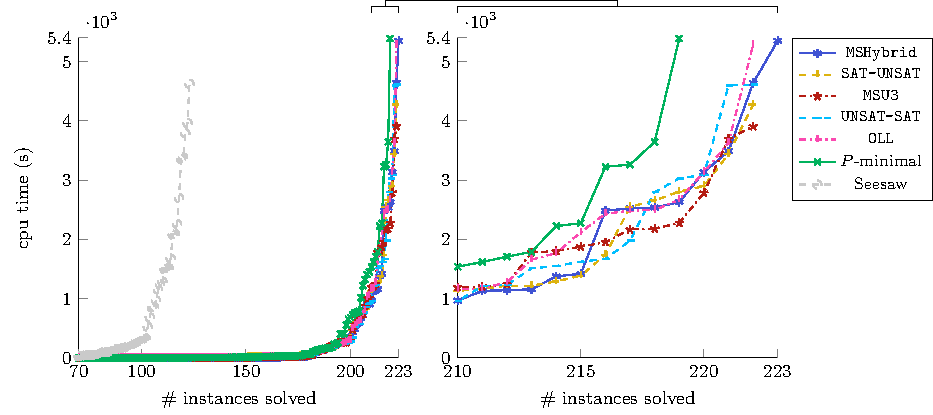
\includegraphics{mlic-cactus-single.pdf}
    \caption{Runtime comparison of $P$-minimal and variants of \algname{} for learning interpretable decision rules;
      enumeration of a single representative solution per Pareto point.
      Plot on the right is zoomed in on the more interesting part of the left plot.
    }\label{fig:mlic-cactus-single}
\end{figure}

% setcover-cactus-single
Next we look at a similar comparison for the bi-objective set covering benchmarks.
In this comparison, Seesaw is not included since it cannot be feasibly instantiated for this task.
\Cref{fig:setcover-cactus-single} shows the number of solved instances per individual time limit for the two generated sets of bi-objective set covering instances.
Here again \msh{} is the best-performing variant of \algname{}, considerably outperforming $P$-minimal:
$P$-minimal solved 71 (respectively 38) fixed element probability (respectively set cardinality) instances, whereas \msh{} solved 83 (respectively 40) instances.
For this application, not all variants of \algname{} outperformed $P$-minimal:
\msu{} and \oll{} were outperformed for both instance variants while \satunsat{} and \unsatsat{} were only outperformed for the instances generated with fixed set cardinality.

% setcover-cactus-single
\begin{figure}
    \centering
    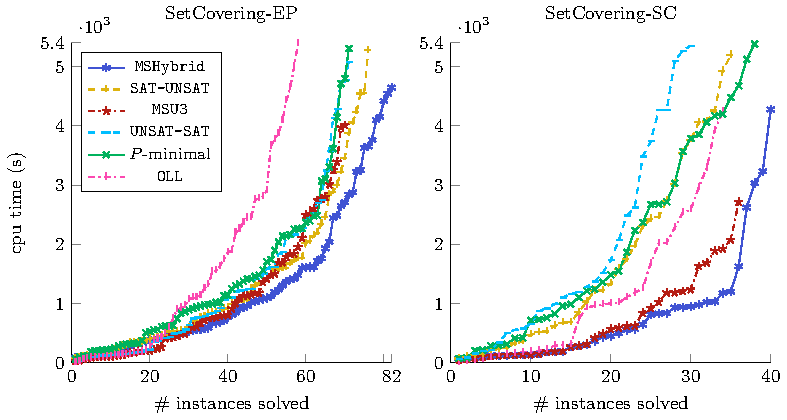
\includegraphics{setcover-cactus-single.pdf}
    \caption{Runtime comparison of $P$-minimal and variants of \algname{} for bi-objective set covering problem;
      enumeration of a single representative solution per Pareto point.
    }\label{fig:setcover-cactus-single}
\end{figure}

% Overall solved instances and best-performaning
The numbers of solved instances for all approaches (except Seesaw) are summarized in \cref{tab:nsolved-single}.
The best-performing approach for each benchmark is highlighted in bold font.
\msh{} is the best-performing \algname{} variant overall, outperforming $P$-minimal in all cases.
For more details, \cref{fig:msh-scatter-single} shows a per-instance runtime comparison between \msh{} and $P$-minimal.
We note that $P$-minimal did not uniquely solve any instance.
In general, \msh{} was outperformed by $P$-minimal on only 31 instances while \msh{} solved 297 instances in less time.

% nsolved-single
\begin{table}
  \centering
  \caption{Solved instances by approach and benchmark family;
    enumeration of a single representative per Pareto point.
  }\label{tab:nsolved-single}
  \begin{tabular}{@{}lrrrrrr@{}}
    \toprule
    Instance Type & \satunsat{} & \unsatsat{} & \msu{} & \oll{} & \msh{} & $P$-minimal \\
    \midrule
    Decision Rules & \textbf{223} & \textbf{223} & \textbf{223} & 222 & \textbf{223} & 219 \\
    \scep{} & 77 & 71 & 71 & 58 & \textbf{83} & 71 \\
    \scsc{} & 35 & 29 & 36 & 34 & \textbf{40} & 38 \\
    \bottomrule
  \end{tabular}
\end{table}

% msh-scatter-single
\begin{figure}
  \centering
  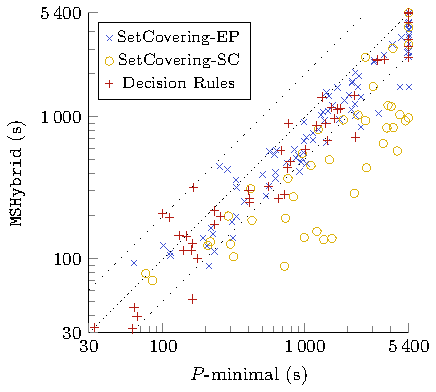
\includegraphics{all-datasets-msh-scatter-log-single.pdf}
  \caption{Runtime comparison between $P$-minimal and \algname{} in the \msh{} variant;
    enumeration of a single representative per Pareto point.
  }\label{fig:msh-scatter-single}
\end{figure}

\TODO{Include time per objective.}

\subsection{Enumerating All Pareto-Optimal Solutions}

% mlic-cactus-multi
Next we compare the performance for learning all Pareto-optimal interpretable decision rules.
\Cref{fig:mlic-cactus-multi} shows the results for this task, presented in the same way as in \cref{fig:mlic-cactus-single}.
For this task, the \algname{} variants \satunsat{}, \unsatsat{}, \msu{} and \msh{} all performed the best, solving 215 instances each.
With this, they outperform $P$-minimal, which only solved 213 instances.
For this task, the \oll{} variant of \algname{} solves the same number of instances as $P$-minimal.
Note that the Seesaw configuration included in \cref{fig:mlic-cactus-multi} does not strictly solve the same task as the other.
As mentioned previously, Seesaw cannot be easily extended to enumerate all Pareto-optimal solutions, we still include it here to show that even when solving the potentially more complex task of enumerating all Pareto-optimal solutions, the other approaches clearly outperform Seesaw.

% mlic-cactus-multi
\begin{figure}
  \centering
  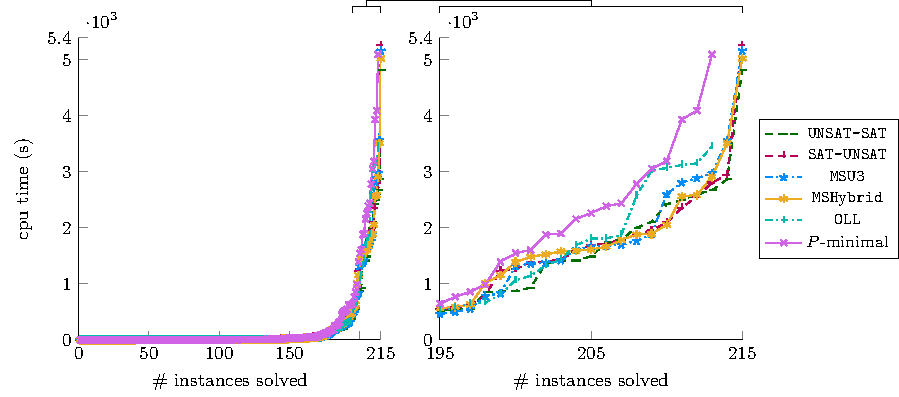
\includegraphics{mlic-cactus.pdf}
  \caption{Runtime comparison of $P$-minimal and variants of \algname{} for learning interpretable decision rules;
    enumeration of all Pareto-optimal solutions.
    Plot on the right is zoomed in on the more interesting part of the left plot.
  }\label{fig:mlic-cactus-multi}
\end{figure}

% setcover-cactus-multi
Looking at the same comparison for bi-objective set covering, we can see in \cref{fig:setcover-cactus-multi} that \msh{} was the best-performing approach also here.
For the instances with fixed set cardinality, all \algname{} variants solved at least as many instances as $P$-minimal, for the instances with fixed element probability only \oll{} was outperformed.
The best-performing variant, \msh{}, solved 81 (respectively 40) of the fixed element probability (respectively set cardinality) instances while $P$-minimal only solved 68 (respectively 26).

% setcover-cactus-multi
\begin{figure}
  \centering
  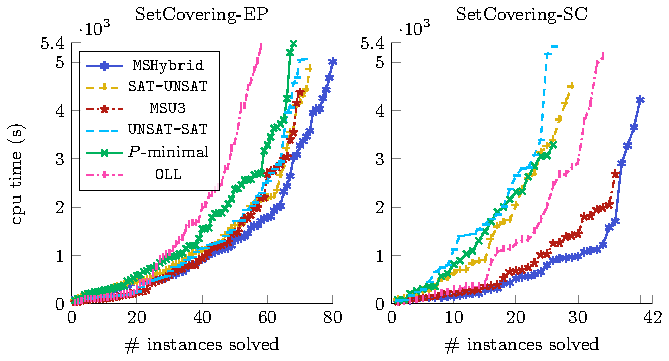
\includegraphics{setcover-cactus.pdf}
  \caption{Runtime comparison of $P$-minimal and variants of \algname{} for bi-objective set covering problem;
    enumeration of all Pareto-optimal solutions.
  }\label{fig:setcover-cactus-multi}
\end{figure}

% Overall solved instances and best-performing
\Cref{tab:nsolved-multi} summarizes the number of solved instances for all approaches applicable to this task.
The best-performing approach for each benchmark is highlighted in bold font.
It can be seen that \msh{} is the best-performing approach for this task as well.
A per-instance runtime comparison between \msh{} and $P$-minimal for the task of enumerating all Pareto-optimal solutions can be seen in \cref{fig:combined-msh-scatter-single-multi} (left).
$P$-minimal did also not uniquely solve any instance for enumerating all Pareto-optimal solutions.
Furthermore, \msh{} was outperformed by $P$-minimal on 71 instances while \msh{} solved 257 instances faster.

% nsolved-multi
\begin{table}
  \centering
  \caption{Solved instances by approach and benchmark family;
    enumeration of all Pareto-optimal solutions.
  }\label{tab:nsolved-multi}
  \begin{tabular}{@{}lrrrrrr@{}}
    \toprule
    Instance Type & \satunsat{} & \unsatsat{} & \msu{} & \oll{} & \msh{} & $P$-minimal \\
    \midrule
    Decision Rules & \textbf{215} & \textbf{215} & \textbf{215} & 213 & \textbf{215} & 213 \\
    \scep{} & 75 & 71 & 70 & 58 & \textbf{81} & 68 \\
    \scsc{} & 35 & 29 & 36 & 34 & \textbf{40} & 26 \\
    \bottomrule
  \end{tabular}
\end{table}

% Single multi comparison
Comparing the number of solved instances between \cref{tab:nsolved-single} and \cref{tab:nsolved-multi}, we can see that the performance difference between \algname{} and $P$-minimal is greater when enumerating all Pareto-optimal solutions.
Furthermore, \cref{fig:combined-msh-scatter-single-multi} (right) shows a runtime comparison between enumerating a single representative solution per Pareto point and enumerating all Pareto-optimal solutions with \msh{}.
Overall, the approach scales well also for the latter task, although there understandable is an overhead when the number of solutions required to be enumerated grows significantly;
this is the case for learning interpretable decision rules, where some instances have more than 10\,000 solutions per Pareto point.
This is in contrast to the set covering instances, which tend to have only a single (of few) solutions per Pareto point.
The fewer solutions per Pareto point for the set covering instances can be explained by the weighted objectives which make it significantly less likely that two distinct solutions have identical objective function values.

% combined-msh-scatter-single-multi
\begin{figure}
  \centering
  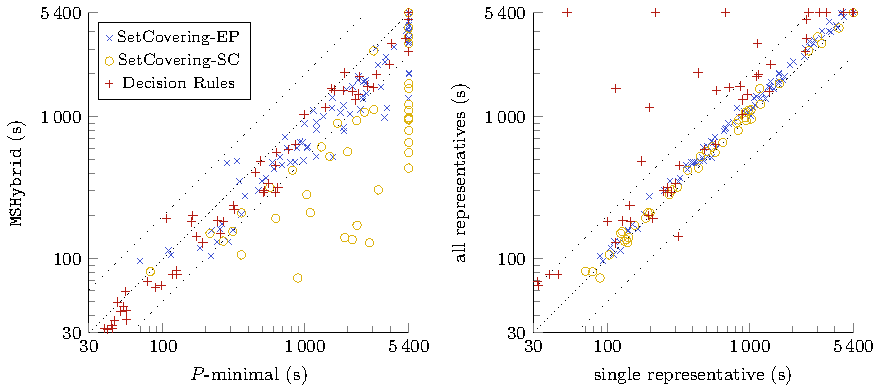
\includegraphics{all-datasets-combined-msh-and-enumeration.pdf}
  \caption{Left: Runtime comparison between $P$-minimal and \algname{} in the \msh{} variant; 
    enumeration of all Pareto-optimal solutions.
    Right: Runtime comparison between enumerating a single representative vs.\ all solutions per Pareto point with \msh{}.}\label{fig:combined-msh-scatter-single-multi}
\end{figure}

\subsection{Impact of Refinements}

% Lazily building the totalizer for the decreasing objective
Finally, we evaluated the impact of the refinements proposed in \cref{sec:refinements} on the runtime efficiency of the best-performing approach, \msh{}.
As the first refinement considered, we evaluate the impact of lazily building the totalizer for the decreasing objective.
\Cref{fig:refinements-1} (left) shows a runtime comparison between \msh{} with and without lazy building of $\tot(\Obj_\dec)$.
It can be seen that for learning interpretable decision rules, this refinement has no evident impact.
This is to be expected since the for these benchmarks, the literals from $\Obj_\dec$ do not appear in $\Obj_\inc$, so $\tot(\Obj_\dec)$ cannot be lazily built.
For the set covering instances with fixed element probability, the impact of this refinement is small and tends to be slightly negative for most instances.
For fixed set cardinality set covering however, we see a strong positive effect.

% Core minimization
Next, we look at the impact of different core minimization strategies.
By default, \msh{} employs heuristic core minimization, in \cref{fig:refinements-1} (right), the performance of this configuration is compared to using exact core minimization instead.
Heuristic core minimization appears to have a positive effect for the task of learning interpretable decision rules as well as for harder set covering instances.
However, the differences to exact minimization are smaller than those regarding lazily building $\tot(\Obj_\dec)$.

% refinements-1
\begin{figure}
    \centering
    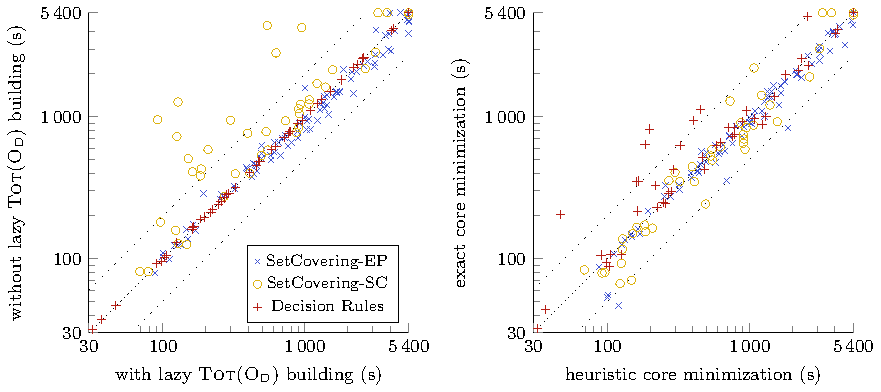
\includegraphics{all-datasets-chosen-refinements-1.pdf}
    \caption{Instance runtime comparisons for the two refinements lazily building the totalizer for the decreasing objective (left) and exact core minimization (right).}\label{fig:refinements-1}
\end{figure}

% Blocking dominated solutions
\Cref{fig:refinements-2} (left) shows the effect of adding the blocking of dominated solutions in the \satunsat{} phase of \msh{}.
The impact of this refinement is miniscule on all benchmarks, however, there are three instances of the set covering benchmarks with fixed element probability that were only solved when not blocking dominated solutions, giving this configuration a slight advantage.
On the decision rule instances, slight positive effects of the refinement can be seen, however, the effect is not strong enough to enable solving of an additional instance.

% Disjoint phase
As the last refinement considered, we look at adding a disjoint phase to the \msu{} phase of \msh{}.
\Cref{fig:refinements-2} shows the impact of adding this refinement to the default configuration of \msh{}.
It can be seen that the effect of adding the disjoint phase does also not result in a clear positive or negative effect, however the impact per instance varies a lot more compared to the impact of blocking dominated solutions.
The only clear negative impact can be seen on three instances for learning interpretable decision rules.
The strongest outlier is an instance that was solved by the configuration without a disjoint phase in under 700 seconds but could not be solved within the resource constraints by the configuration with a disjoint phase.

% refinements-2
\begin{figure}
    \centering
    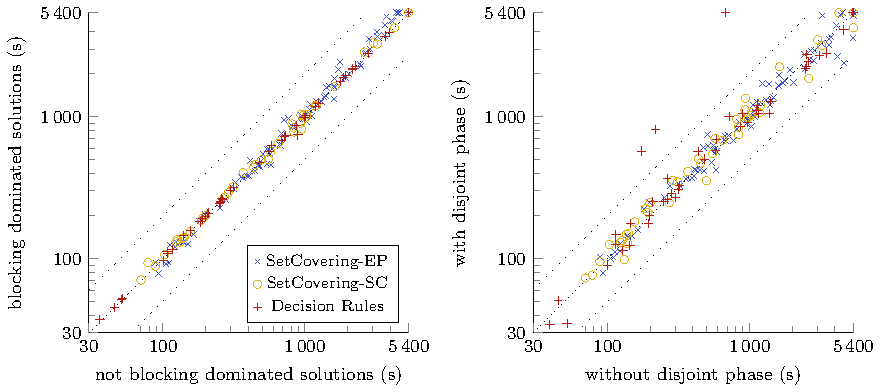
\includegraphics{all-datasets-chosen-refinements-2.pdf}
    \caption{Instance runtime comparisons for the two refinements blocking dominated solutions (left) and disjoint core extraction (right).}\label{fig:refinements-2}
\end{figure}
\chapter{Conclusions\label{chap:conclusion}}

% Recap of contribution
In this thesis, we presented \algname{}, an algorithm for exact bi-objective optimization under Pareto optimality.
The structured search procedure of \algname{} builds on solving algorithms for maximum satisfiability and makes incremental use of a solver for propositional satisfiability.
It can solve three different tasks for \NP-hard optimization problems encoded into propositional logic:
finding a single Pareto-optimal solution, one representative solution for each Pareto point, and all Pareto-optimal solutions.

% Results of BiOptSat variants comparing to competitors
We presented five variants of \algname{}, based on different MaxSAT algorithms: \satunsat{}, \unsatsat{}, \msu{}, \oll{} and \msh{}.
These five variants were evaluated on two benchmark domains: learning interpretable decision rules~\autocite{DBLP:conf/cp/MaliotovM18} and bi-objective set covering.
In the empirical evaluation we found that the \msh{} variant did not only outperform all other four variants of \algname{} but also all three competitors, $P$-minimal~\autocite{DBLP:conf/cp/SohBTB17}, ParetoMCS~\autocite{DBLP:conf/ijcai/Terra-NevesLM18a}, and Seesaw~\autocite{DBLP:conf/cp/JanotaMSM21}.
Other variants of \algname{} also outperformed the competitors in many cases.
The good performance of \algname{} is in part because of the incremental use of the SAT solver, but mainly due to the structured nature of the search performed by the algorithm.
\msh{} in particular achieves good performance by combining advantages from the MSU3 and the SAT-UNSAT MaxSAT algorithms.
Evaluation was done for the two tasks of finding one representative solution for each Pareto point, and for enumerating all Pareto-optimal solutions.
The advantage of \algname{} over its competitors is slightly more pronounced when enumerating all Pareto-optimal solutions.

% Results of refinements
Going beyond evaluating variants of \algname{}, we also evaluated refinements to the best performing variant, \msh{}.
The refinements we found to be most impactful were lazily building the totalizer for the decreasing objective when the two objectives share literals, and heuristic core minimization.
Other refinements that did not show a significant impact on performance are blocking of solutions dominated by candidates found during the search and adding a disjoint core-extraction phase.

% Future work
Going beyond the work presented in this thesis, \algname{} could be further improved and evaluated.
Evaluating the performance of \algname{} as well for the task of finding a single Pareto-optimal solution is interesting future work.
Furthermore, for weighted problem instances, the used totalizer encoding could be replaced by the improved generalized totalizer encoding~\autocite{DBLP:conf/cp/0001MM15}.
This encoding is smaller in the case that the subset sums of the cost values do not include every possible value in the range from 1 to the upper bound $k$.
For this reason, this change of cardinality constraint encoding could improve the performance of \algname{} on weighted instances.
Furthermore, a better understanding for what objective should be chosen as increasing to achieve the best performance remains an interesting open question.

%%%%%%%%%%%%%%%%%%%%%%%%%%%%%%%%%%%%%%%%%%%%%%%%%%%%%%%%%
%\cleardoublepage                          %fixes the position of bibliography in bookmarks
%\phantomsection
\addcontentsline{toc}{chapter}{\bibname}  % This lines adds the bibliography to the ToC
\printbibliography

%%%%%%%%%%%%%%%%%%%%%%%%%%%%%%%%%%%%%%%%%%%%%%%%%%%%%%%%%
\backmatter
\begin{appendices}

%% A sample Appendix
\appendix{Datasets Used for Decision Rule Learning\label{appendix:datasets}}

\Cref{tab:datasets} summarizes the datasets used in the empirical evaluations, including their origin and statistics, as well as the sizes of CNF formulas obtained from them with the encoding from~\textcite{DBLP:conf/cp/MaliotovM18}.
The original files were downloaded from the UCI Machine Learning Repository~\autocite{UciMlr} and from Kaggle ({\small\url{https://www.kaggle.com}}).
Links to the original datasets as well as the files we used will be made available online upon publication.
We randomly and independently sampled subsets of $\nsamp\in\{50,100,1000,5000,10000\}$ data samples from the datasets, four of each size (when applicable), resulting in a         
total of 372 datasets, and discretized the data as in~\autocite{DBLP:conf/cp/MaliotovM18}:
categorical features are one-hot encoded, continuous features discretized by comparing to a collection of thresholds. 

In addition to the name and the source of the datasets, the table shows the number of data samples as well as the number of features before and after discretization.
The last two columns give some statistics about the formulas generated with the encoding from~\textcite{DBLP:conf/cp/MaliotovM18} for two clauses based on the full datasets.
We report both the number of clauses and the number of variables in these formulas.
In case the 16-GB memory limit was already reached, and the run terminated before the formula was created, these two columns are marked with ``memout''.
Note that the memouts are for the full datasets; also for those datasets sampled subsets were used in the experiments.

For the decision rule instances, the instance that took the longest time to solve that did not time out for the \msh{} variant was a subset of 100 examples of the Connect 4 dataset.
The formula of this dataset has 3362 variables and 42621 clauses.
The largest instance in terms of the number of examples that our algorithm was able to find a representative for every Pareto-point for was a subset of the Travel Insurance dataset with 10000 samples.
When looking at the number of features, the largest solvable dataset was a subset of the Twitter dataset with 50 examples and 1511 discretized features.

\begin{sidewaystable}
    \centering
    \caption{The datasets used in the decision rule experiments and some summary statistics about them and the encoded formulas created from them.}\label{tab:datasets}
    {\small
    \begin{tabular}{@{}llrrrrr@{}}
        \toprule
        Dataset & Source & \# examples & \# features & \# disc. feat. & \# clauses ($10^6$) & \# vars ($10^3$) \\
        \midrule
        Adult & UCI & 32561 & 14 & 144 & 226 & 589 \\
        Bank Marketing & UCI & 45211 & 16 & 88 & 227 & 840 \\
        Banknote Authentication & UCI & 1372 & 4 & 16 & 0.67 & 18.7\\
        Connect 4 & UCI & 67557 & 42 & 126 & \multicolumn{2}{c}{memout} \\
        Default of Credit Card Clients & UCI & 30000 & 23 & 110 & 178 & 539 \\
        Dota 2 Games Results & UCI & 92650 & 115 & 345 & \multicolumn{2}{c}{memout}\\
        FIFA 2018 Man of the Match & Kaggle & 128 & 26 & 106 & 0.034 & 3.3 \\
        Heart Disease & Kaggle & 303 & 13 & 31 & 0.044 & 3.9 \\
        Indian Liver Patient Dataset & UCI & 583 & 10 & 14 & 0.096 & 7.3 \\
        Ionosphere & UCI & 351 & 33 & 144 & 0.11 & 6.8 \\
        Iris & UCI & 150 & 4 & 11 & 0.0087 & 1.7 \\
        MAGIC Gamma Telescope & UCI & 19020 & 10 & 79 & 105 & 330 \\
        Medical Hospital Readmissions & Kaggle & 25000 & 64 & 125 & 222 & 445 \\
        Mushroom & UCI & 8124 & 22 & 115 & 24.5 & 132 \\
        Parkinsons & UCI & 195 & 22 & 51 & 0.028 & 2.9 \\
        Pima Indians Diabetes & Kaggle & 768 & 8 & 30 & 0.19 & 10 \\
        Skin Segmentation & UCI & 245057 & 3 & 119 & \multicolumn{2}{c}{memout} \\
        Tic-Tac-Toe Endgame & UCI & 958 & 9 & 27 & 422 & 13 \\
        Buzz in Social Media (Toms Hardware) & UCI & 28179 & 96 & 910 & 220 & 525 \\
        Buzz in Social Media (Twitter) & UCI & 49999 & 77 & 1511 & \multicolumn{2}{c}{memout} \\
        Blood Transfusion Service Center & UCI & 748 & 4 & 6 & 0.13 & 9.5 \\
        Travel Insurance & Kaggle & 63326 & 10 & 211 & 50 & 1205 \\
        Wisconsin Diagnostic Breast Cancer & UCI & 569 & 30 & 88 & 0.14 & 8.5 \\
        Rain in Australia & Kaggle & 107696 & 16 & 141 & \multicolumn{2}{c}{memout} \\
        \bottomrule
    \end{tabular}
    }
\end{sidewaystable}

\end{appendices}
%%%%%%%%%%%%%%%%%%%%%%%%%%%%%%%%%%%%%%%%%%%%%%%%%%%%%%%%%

\end{document}
